\documentclass{beamer}\usepackage[]{graphicx}\usepackage[]{color}
% maxwidth is the original width if it is less than linewidth
% otherwise use linewidth (to make sure the graphics do not exceed the margin)
\makeatletter
\def\maxwidth{ %
  \ifdim\Gin@nat@width>\linewidth
    \linewidth
  \else
    \Gin@nat@width
  \fi
}
\makeatother

\definecolor{fgcolor}{rgb}{0.345, 0.345, 0.345}
\newcommand{\hlnum}[1]{\textcolor[rgb]{0.686,0.059,0.569}{#1}}%
\newcommand{\hlstr}[1]{\textcolor[rgb]{0.192,0.494,0.8}{#1}}%
\newcommand{\hlcom}[1]{\textcolor[rgb]{0.678,0.584,0.686}{\textit{#1}}}%
\newcommand{\hlopt}[1]{\textcolor[rgb]{0,0,0}{#1}}%
\newcommand{\hlstd}[1]{\textcolor[rgb]{0.345,0.345,0.345}{#1}}%
\newcommand{\hlkwa}[1]{\textcolor[rgb]{0.161,0.373,0.58}{\textbf{#1}}}%
\newcommand{\hlkwb}[1]{\textcolor[rgb]{0.69,0.353,0.396}{#1}}%
\newcommand{\hlkwc}[1]{\textcolor[rgb]{0.333,0.667,0.333}{#1}}%
\newcommand{\hlkwd}[1]{\textcolor[rgb]{0.737,0.353,0.396}{\textbf{#1}}}%
\let\hlipl\hlkwb

\usepackage{framed}
\makeatletter
\newenvironment{kframe}{%
 \def\at@end@of@kframe{}%
 \ifinner\ifhmode%
  \def\at@end@of@kframe{\end{minipage}}%
  \begin{minipage}{\columnwidth}%
 \fi\fi%
 \def\FrameCommand##1{\hskip\@totalleftmargin \hskip-\fboxsep
 \colorbox{shadecolor}{##1}\hskip-\fboxsep
     % There is no \\@totalrightmargin, so:
     \hskip-\linewidth \hskip-\@totalleftmargin \hskip\columnwidth}%
 \MakeFramed {\advance\hsize-\width
   \@totalleftmargin\z@ \linewidth\hsize
   \@setminipage}}%
 {\par\unskip\endMakeFramed%
 \at@end@of@kframe}
\makeatother

\definecolor{shadecolor}{rgb}{.97, .97, .97}
\definecolor{messagecolor}{rgb}{0, 0, 0}
\definecolor{warningcolor}{rgb}{1, 0, 1}
\definecolor{errorcolor}{rgb}{1, 0, 0}
\newenvironment{knitrout}{}{} % an empty environment to be redefined in TeX

\usepackage{alltt}

\usepackage{animate}

\def\currentCourse{Data anaysis and Unsupervised Learning}
\def\currentInstitute{MAP 573, 2020 -- Julien Chiquet}
\def\currentLogo{../common_figs/logo_X}
\def\currentDate{\'Ecole Polytechnique, Autumn semester, 2020}
\def\currentChapter{Clustering: distance-based methods}


% THEME BEAMER
\usepackage{../beamer_theme}

\graphicspath{{figures/},{../common_figs/}}

\usepackage{multirow}
\usepackage{tikz}
\usepackage[vlined]{algorithm2e}

\pgfdeclareimage[width=.5cm]{computer}{computer.png}

% \usetikzlibrary{calc,shapes,backgrounds,arrows,automata,shadows,positioning}
% \tikzstyle{every state}=[fill=red,draw=none,scale=0.7,font=\small,text=white]
% \tikzstyle{every edge}=[-,shorten >=1pt,auto,thin,draw]
% \tikzstyle{alertstate}=[fill=bleu]
% \definecolor{genecolor}{RGB}{94,135,173}

\title{\currentCourse}

\subtitle{\huge\currentChapter\normalsize}

\institute{\currentInstitute}

\date{\currentDate}



\AtBeginSection{
  \begin{frame}<beamer>
    \frametitle{Outline}
    \framesubtitle{\insertpart}
    \tableofcontents[currentsection,currentsubsection, subsectionstyle=show/shaded/hide]  
  \end{frame}
}

\AtBeginSubsection{
  \begin{frame}<beamer>
    \frametitle{Outline}
    \framesubtitle{\insertpart}
    \tableofcontents[currentsection,currentsubsection, subsectionstyle=show/shaded/hide]  
  \end{frame}
}

\AtBeginSubsubsection{
  \begin{frame}<beamer>
    \frametitle{Outline}
    \framesubtitle{\insertpart}
    \tableofcontents[currentsection,currentsubsection, subsectionstyle=show/shaded/hide]  
  \end{frame}
}

\newcommand{\dotitlepage}{%
  \begin{frame}
    \titlepage
    \vfill
    \begin{center}
        \scriptsize\url{https://jchiquet.github.io/MAP573}
    \end{center}
    \vfill
    \includegraphics[width=2cm]{\currentLogo}\hfill
    \includegraphics[width=2.5cm]{logo_inra}
  \end{frame}
  %
}

\newcommand{\dotoc}{%
  \begin{frame}
    \frametitle{Outline}
    \tableofcontents[currentsection,
    sectionstyle=show/show,
    subsectionstyle=hide]
  \end{frame}
  %
}

\usetikzlibrary{calc,shapes,backgrounds,arrows,automata,shadows,positioning}

\graphicspath{{figures/}}
\IfFileExists{upquote.sty}{\usepackage{upquote}}{}
\begin{document}

\dotitlepage

%% ====================================================================
\part{Introduction}
%% ====================================================================

\begin{frame}[fragile]
  \frametitle{Packages required for reproducing the slides}
  
\begin{knitrout}\scriptsize
\definecolor{shadecolor}{rgb}{0.969, 0.969, 0.969}\color{fgcolor}\begin{kframe}
\begin{alltt}
\hlkwd{library}\hlstd{(tidyverse)}  \hlcom{# opinionated collection of packages for data manipulation}
\hlkwd{library}\hlstd{(corrplot)}   \hlcom{# fancy plots of matrices as images}
\hlkwd{library}\hlstd{(GGally)}     \hlcom{# extension to ggplot vizualization system}
\hlkwd{library}\hlstd{(FactoMineR)} \hlcom{# PCA and oter linear method for dimension reduction}
\hlkwd{library}\hlstd{(factoextra)} \hlcom{# fancy plotting for FactoMineR output}
\hlkwd{library}\hlstd{(kernlab)}    \hlcom{# Kernel-based methods, among which spectral-clustering}
\hlkwd{library}\hlstd{(aricode)}    \hlcom{# fast computation of clustering measures}
\hlkwd{library}\hlstd{(animation)}  \hlcom{# kmeans animation slides}
\hlkwd{library}\hlstd{(igraph)}     \hlcom{# graph manipulation}
\hlkwd{theme_set}\hlstd{(}\hlkwd{theme_bw}\hlstd{())} \hlcom{# plots themes}
\end{alltt}
\end{kframe}
\end{knitrout}
  
\end{frame}

\begin{frame}[fragile]
  \frametitle{Companion data set}
  \framesubtitle{Morphological Measurements on Leptograpsus Crabs}
  
\begin{block}{Description}
\small The crabs data frame has 200 rows and 8 columns, describing 5 morphological measurements on 50 crabs each of two colour forms and both sexes, of the species \textit{Leptograpsus variegatus} collected at Fremantle, W. Australia.
\end{block}
  
\begin{knitrout}\scriptsize
\definecolor{shadecolor}{rgb}{0.969, 0.969, 0.969}\color{fgcolor}\begin{kframe}
\begin{alltt}
\hlstd{crabs} \hlkwb{<-} \hlstd{MASS}\hlopt{::}\hlstd{crabs} \hlopt \hlkwd{select}\hlstd{(}\hlopt{-}\hlstd{index)} \hlopt
  \hlkwd{rename}\hlstd{(}\hlkwc{sex} \hlstd{= sex,}
         \hlkwc{species}         \hlstd{= sp,}
         \hlkwc{frontal_lob}     \hlstd{= FL,}
         \hlkwc{rear_width}      \hlstd{= RW,}
         \hlkwc{carapace_length} \hlstd{= CL,}
         \hlkwc{carapace_width}  \hlstd{= CW,}
         \hlkwc{body_depth}      \hlstd{= BD)}
\hlstd{crabs} \hlopt \hlkwd{select}\hlstd{(sex, species)} \hlopt \hlkwd{summary}\hlstd{()} \hlopt \hlstd{knitr}\hlopt{::}\hlkwd{kable}\hlstd{(}\hlstr{"latex"}\hlstd{)}
\end{alltt}
\end{kframe}
\begin{tabular}{l|l|l}
\hline
  & sex & species\\
\hline
 & F:100 & B:100\\
\hline
 & M:100 & O:100\\
\hline
\end{tabular}


\end{knitrout}
\end{frame}

\begin{frame}[fragile]
  \frametitle{Companion data set II}
  \framesubtitle{Pairs plot of attributes}

\begin{knitrout}\scriptsize
\definecolor{shadecolor}{rgb}{0.969, 0.969, 0.969}\color{fgcolor}\begin{kframe}
\begin{alltt}
\hlkwd{ggpairs}\hlstd{(crabs,} \hlkwc{columns} \hlstd{=} \hlnum{3}\hlopt{:}\hlnum{7}\hlstd{,} \hlkwd{aes}\hlstd{(}\hlkwc{colour} \hlstd{=} \hlkwd{paste}\hlstd{(crabs}\hlopt{$}\hlstd{species, crabs}\hlopt{$}\hlstd{sex)))}
\end{alltt}
\end{kframe}
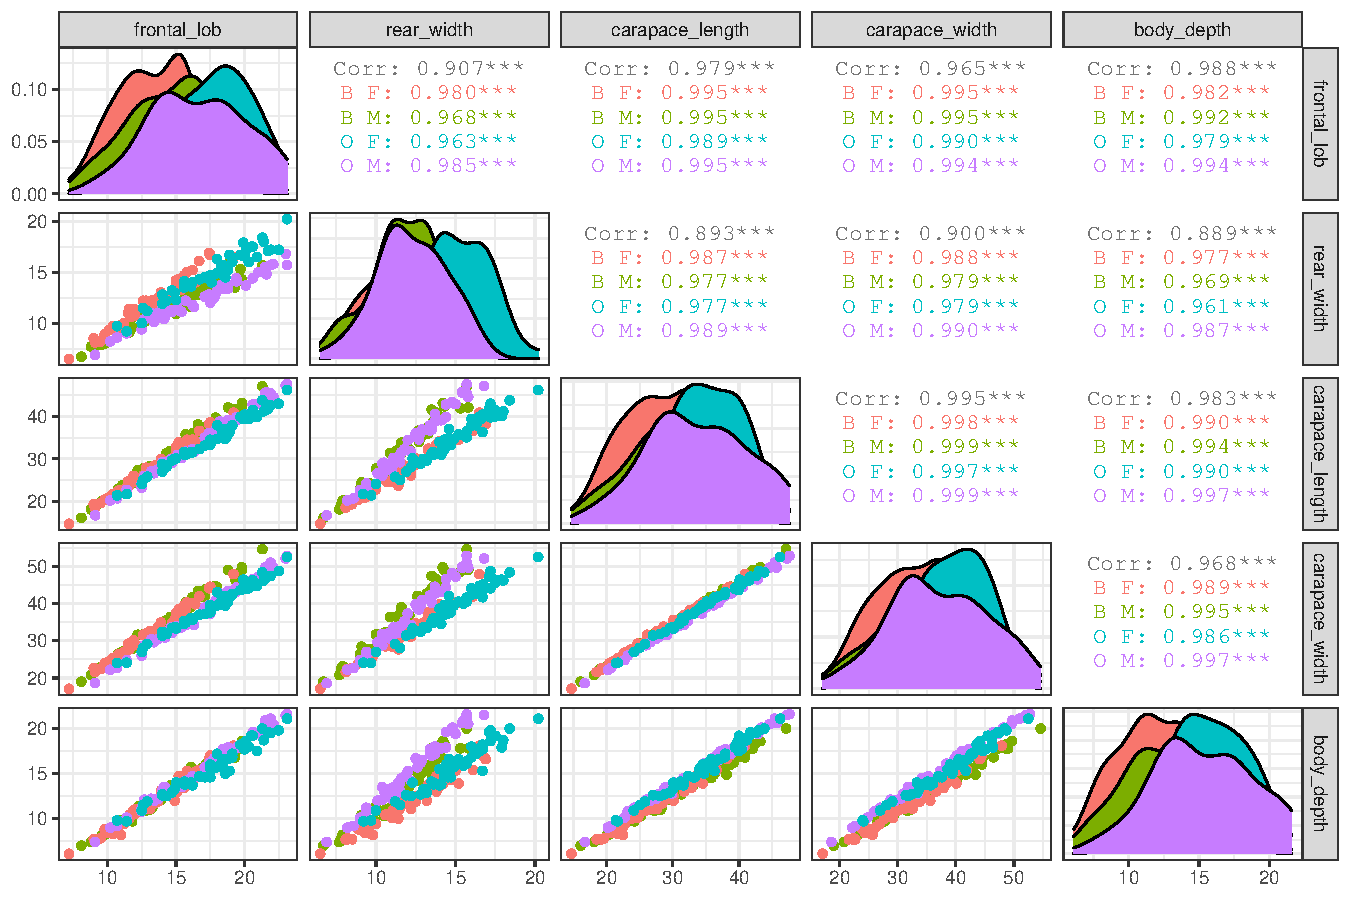
\includegraphics[width=.8\textwidth]{figures/crabs_attributes-1} 

\end{knitrout}
\end{frame}

\begin{frame}[fragile]
  \frametitle{Companion data set III}
  \framesubtitle{PCA on the attributes}

\begin{knitrout}\scriptsize
\definecolor{shadecolor}{rgb}{0.969, 0.969, 0.969}\color{fgcolor}\begin{kframe}
\begin{alltt}
\hlkwd{select}\hlstd{(crabs,} \hlopt{-}\hlstd{species,} \hlopt{-}\hlstd{sex)} \hlopt \hlkwd{PCA}\hlstd{(}\hlkwc{scale.unit} \hlstd{=} \hlnum{FALSE}\hlstd{,} \hlkwc{graph} \hlstd{=} \hlnum{FALSE}\hlstd{)} \hlopt
  \hlkwd{fviz_pca_biplot}\hlstd{(}\hlkwc{axes} \hlstd{=} \hlkwd{c}\hlstd{(}\hlnum{1}\hlstd{,}\hlnum{2}\hlstd{),} \hlkwc{col.ind} \hlstd{=} \hlkwd{paste}\hlstd{(crabs}\hlopt{$}\hlstd{species, crabs}\hlopt{$}\hlstd{sex))}
\end{alltt}
\end{kframe}
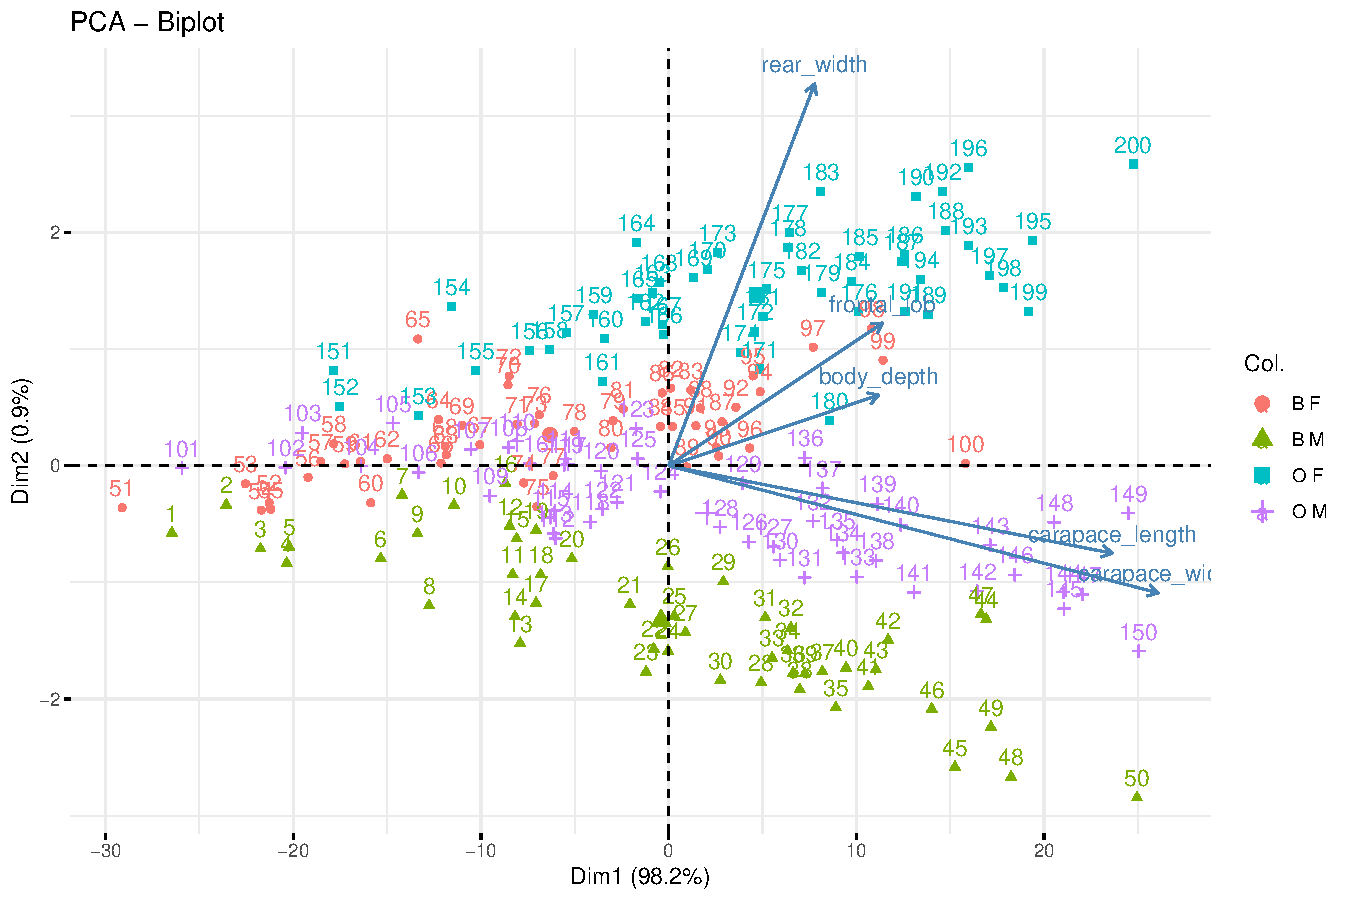
\includegraphics[width=.8\textwidth]{figures/pca_crabs_untransformed-1} 

\end{knitrout}
\end{frame}

\begin{frame}[fragile,allowframebreaks]
  \frametitle{Remove size effect}
  \framesubtitle{Carried by the 1st principal component}

\paragraph{First component}
\begin{equation*}
  \mathbf{f}_1 = \mathbf{X}^c \mathbf{u}_1.
\end{equation*}

We extract the best rank-1 approximation of $\mathbf{X}$ to remove the \textit{size effect}, carried by the first axis, and return to the original space,
\begin{equation*}
  \tilde{\mathbf{X}}^{(1)} = \mathbf{f}_1 \mathbf{u}_1^\top.
\end{equation*}


\begin{knitrout}\scriptsize
\definecolor{shadecolor}{rgb}{0.969, 0.969, 0.969}\color{fgcolor}\begin{kframe}
\begin{alltt}
\hlstd{attributes} \hlkwb{<-} \hlkwd{select}\hlstd{(crabs,} \hlopt{-}\hlstd{sex,} \hlopt{-}\hlstd{species)} \hlopt \hlkwd{as.matrix}\hlstd{()}
\hlstd{u1} \hlkwb{<-} \hlkwd{eigen}\hlstd{(}\hlkwd{cov}\hlstd{(attributes))}\hlopt{$}\hlstd{vectors[,} \hlnum{1}\hlstd{,} \hlkwc{drop} \hlstd{=} \hlnum{FALSE}\hlstd{]}
\hlstd{attributes_rank1} \hlkwb{<-} \hlstd{attributes} \hlopt \hlstd{u1} \hlopt \hlkwd{t}\hlstd{(u1)}
\hlstd{crabs_corrected} \hlkwb{<-} \hlstd{crabs}
\hlstd{crabs_corrected[,} \hlnum{3}\hlopt{:}\hlnum{7}\hlstd{]} \hlkwb{<-} \hlstd{attributes} \hlopt{-} \hlstd{attributes_rank1}
\end{alltt}
\end{kframe}
\end{knitrout}

$\rightsquigarrow$ Axis 1 explains a latent effect, here the size in the case at hand, common to all attributes.

\begin{knitrout}\scriptsize
\definecolor{shadecolor}{rgb}{0.969, 0.969, 0.969}\color{fgcolor}\begin{kframe}
\begin{alltt}
\hlkwd{ggpairs}\hlstd{(crabs_corrected,} \hlkwc{columns} \hlstd{=} \hlnum{3}\hlopt{:}\hlnum{7}\hlstd{,} \hlkwd{aes}\hlstd{(}\hlkwc{colour} \hlstd{=} \hlkwd{paste}\hlstd{(crabs}\hlopt{$}\hlstd{species, crabs}\hlopt{$}\hlstd{sex)))}
\end{alltt}
\end{kframe}
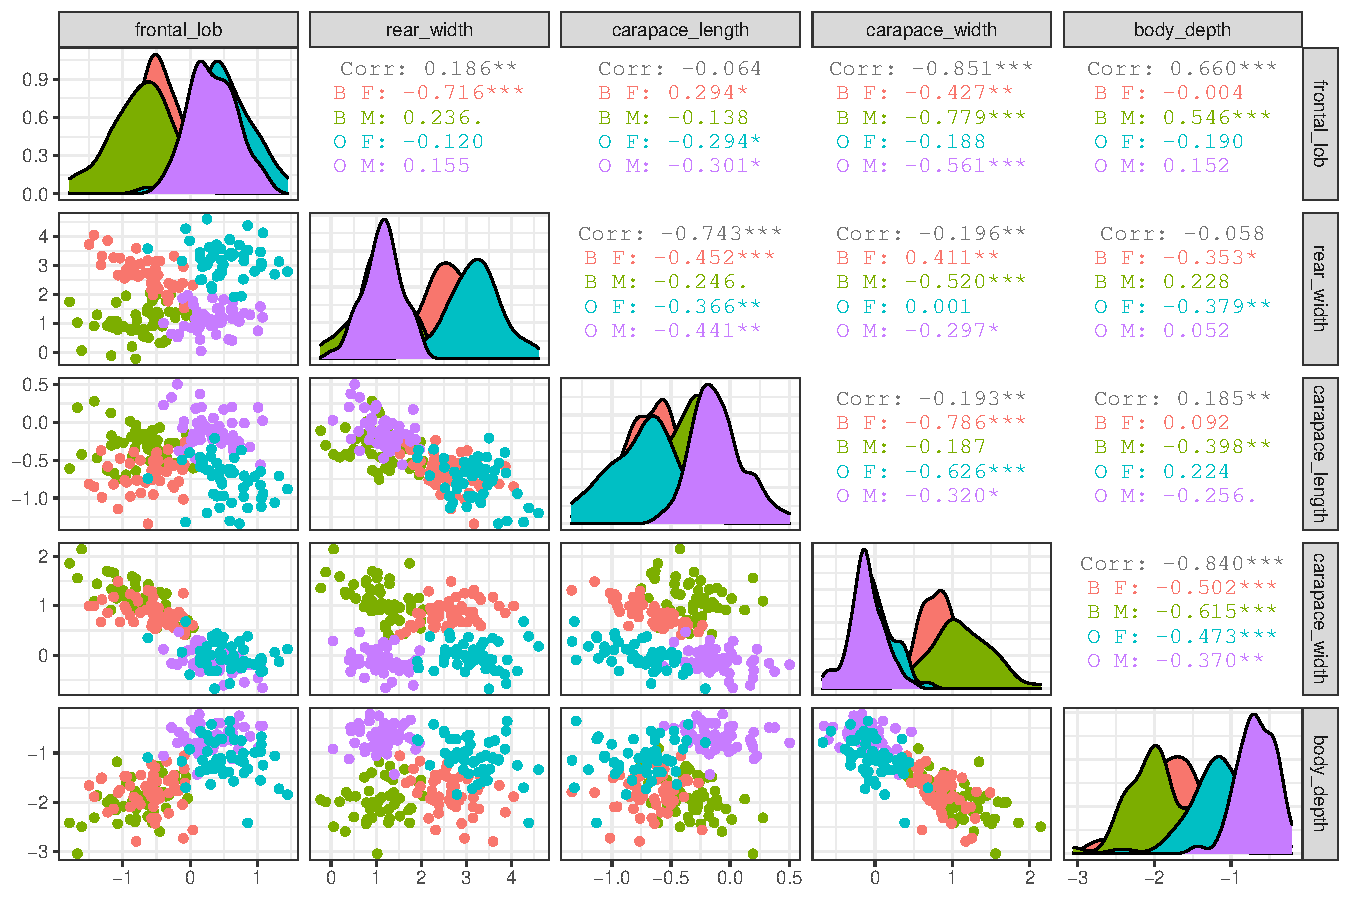
\includegraphics[width=.8\textwidth]{figures/pairs_plot_corrected-1} 

\end{knitrout}

\end{frame}

\begin{frame}[fragile]
  \frametitle{PCA on corrected data}
\begin{knitrout}\scriptsize
\definecolor{shadecolor}{rgb}{0.969, 0.969, 0.969}\color{fgcolor}\begin{kframe}
\begin{alltt}
\hlkwd{select}\hlstd{(crabs_corrected,} \hlopt{-}\hlstd{species,} \hlopt{-}\hlstd{sex)} \hlopt \hlstd{FactoMineR}\hlopt{::}\hlkwd{PCA}\hlstd{(}\hlkwc{graph} \hlstd{=} \hlnum{FALSE}\hlstd{)} \hlopt
\hlkwd{fviz_pca_biplot}\hlstd{(}\hlkwc{col.ind} \hlstd{=} \hlkwd{paste}\hlstd{(crabs_corrected}\hlopt{$}\hlstd{species, crabs_corrected}\hlopt{$}\hlstd{sex))}
\end{alltt}
\end{kframe}
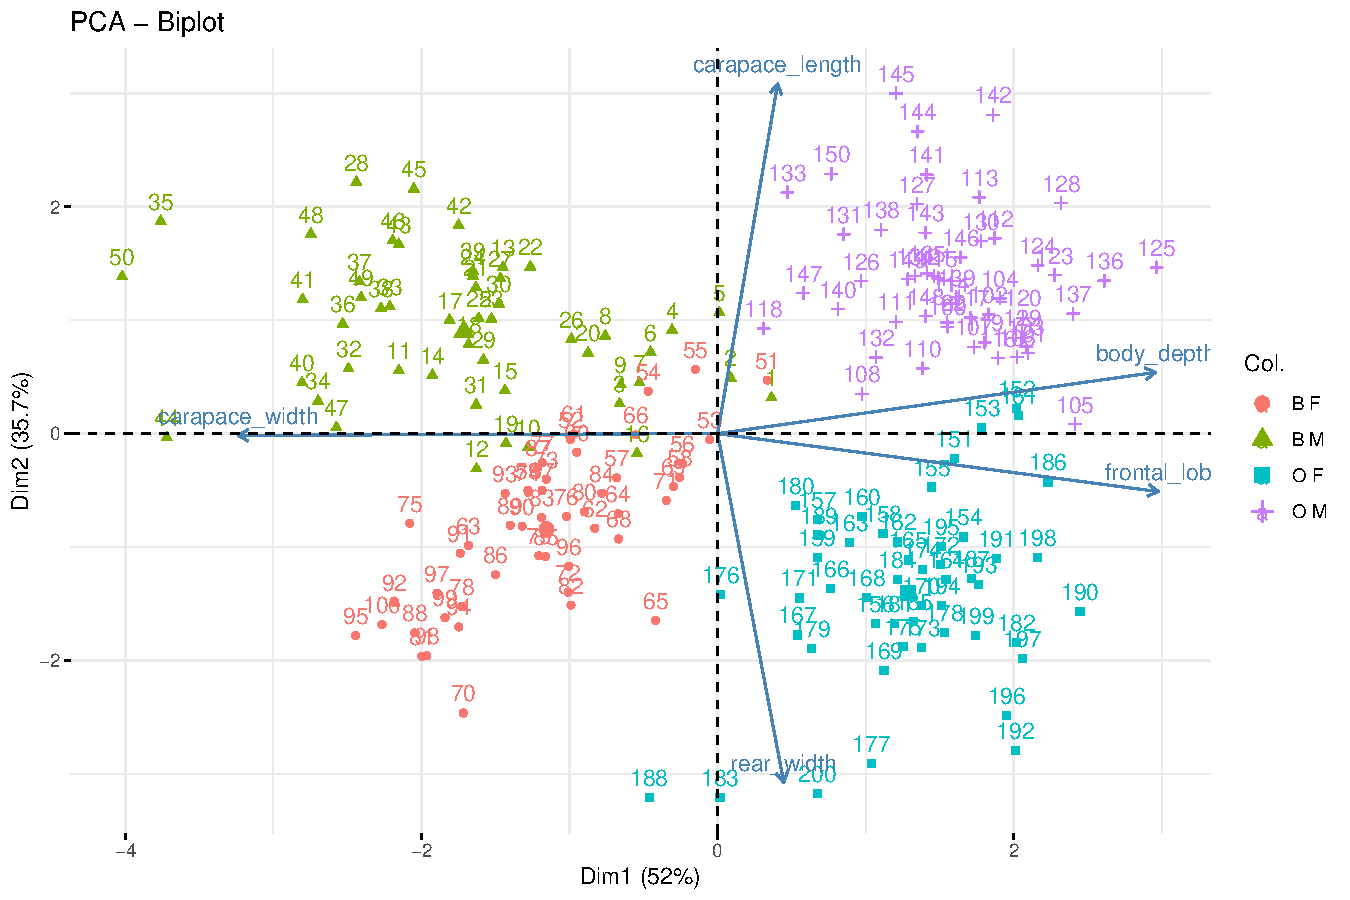
\includegraphics[width=.8\textwidth]{figures/pca_crabs_corrected_biplot-1} 

\end{knitrout}

\end{frame}

\begin{frame}
  \frametitle{Questions}
  \begin{center}
    \begin{enumerate}
      \item Could we automatically identify some grouping (\alert{clustering}) between samples? \medskip
      \item Would this clustering correspond to some known labels (sex, species)? \medskip
      \item Do we need to transform the data before we perform clustering? \medskip
    \end{enumerate}
  \end{center}

\end{frame}

\begin{frame}[label=Clustering1]
  \frametitle{Clustering: general goals}

  \paragraph{Objective}: construct a map 
  \[
    f : \mathcal{D} = \{1,\dots,n\} \mapsto  \{1,\ldots,K\}
  \]
  where $K$ is a fixed number of clusters.
    
  \vfill
    
  \paragraph{Careful! classification $\neq$ clustering}
      \begin{itemize}
      \item Classification presupposes the existence of classes
      \item Clustering labels only elements of the dataset
      \begin{itemize}
      \item[$\rightsquigarrow$] no ground truth (no given labels)
      \item[$\rightsquigarrow$] discovers a structure "natural" to the data
      \item[$\rightsquigarrow$] not necessarily related to a known classification
      \end{itemize}
      \end{itemize}
  
  \vfill

  \paragraph{Motivations}
    \begin{itemize}
    \item describe large masses of data in a simplified way,
    \item structure a set of knowledge,
    \item reveal structures, hidden causes,
    \item use of the groups in further processing, 
    \item \dots
  \end{itemize}

\end{frame}

\begin{frame}[label=Clustering2]

  \frametitle{Clustering: challenges}

    \begin{block}{Clustering quality}
      No obvious measure to define the \alert{quality} of the clusters. Ideas:
      \begin{itemize}
        \item \alert{Inner} homogeneity: samples in the same group should be similar
        \item \alert{Outer} inhomogeneity: samples in different groups should be different
      \end{itemize}
    \end{block}

    \vspace{-.25cm}

    \begin{block}{Number of clusters}
      Choice of the number of clusters $K$ often complex
      \begin{itemize}
        \item No ground truth in unsupervised learning!
        \item Several solutions might be equally good
      \end{itemize}
    \end{block}

    \vspace{-.25cm}

    \begin{block}{Two general approaches}
      \vspace{-.25cm}
      \begin{itemize}
        \item \alert{distance-based}: require a distance/dissimilarity between $\{\bx_i\}$
        \item \alert{model-based}: require assumptions on the distribution $\mathbb{P}$
      \end{itemize}
    \end{block}
    
\end{frame}


%% ====================================================================
\part{Distance-based method}
%% ====================================================================
\begin{frame}
  \partpage
\end{frame}

%% ==========================================================================
%% Clustering: introduction, vocabulary
%% ==========================================================================

%% ==========================================================================
\section{Clustering: introduction}
%% ==========================================================================

\begin{frame}
  \frametitle{Dissimilarity and Distance}

  \paragraph{\it Clustering requires a measure of ressemblance between object}

  \begin{definition}[(dis)similarity]
    Similarity (\textit{resp. Dissimilarity}) measures the ressemblance (\textit{resp. discrepancy}) between objects based on several features. 
  \end{definition}

  For instance, two objects are similar if 
  \begin{itemize}
    \item they share a certain feature
    \item \alert{their features are close according to a measure of proximity}
  \end{itemize}
  
  \vfill
  
  \begin{definition}[distance/metric]<2>
    Dissimilairty can be measuresd by distances, \textit{i.e.} a function $d_{ij}$ between pairs in \{$\bx_i\}$ s.t.
    \vspace{-.25cm}
    \begin{multicols}{2}
    \begin{itemize}
      \item $d_{ij} \geq 0$,
      \item $d_{ij} = 0 \Leftrightarrow \bx_i = \bx_{j}$,
      \item $d_{ij} = d_{ji}$,
      \item $d_{ik} \leq d_{ij} + d_{jk}$.
    \end{itemize}
    \end{multicols}
  \end{definition}

\end{frame}

\begin{frame}
  \frametitle{Classification structures: Partition}

  \paragraph{\it Clustering leads to a grouping (or classification) of individuals into homogeneous classes} 
  \bigskip
  
  We consider two structures to describe this classification: 
  \begin{itemize}
    \item \alert{partitions} and
    \item \alert{hierarchies}.
  \end{itemize}

  \vfill

  \begin{definition}[Partition]
    A partition $\mathcal{P}$ is a decomposition $\mathcal{P} = \{P_1,\dots,P_K\}$ of a finite ensemble $\Omega$ such that
    \begin{itemize}
      \item $P_k \cap P_{k'} = \emptyset$ for any $k\neq k'$
      \item $\bigcup_{k} P_k = \Omega$
    \end{itemize}
    In a set $\Omega = (\bx_1, \dots, \bx_n)$ partitioned into $K$ classes, each element of the set belongs to a
class and only one.
  \end{definition}

\end{frame}

\begin{frame}
  \frametitle{Classification structures: Hierarchy}

  \begin{definition}[Hierarchy]
    A hierarchy $\mathcal{H}$ is a non empty subset of a finite ensemble $\Omega$ such that
    \begin{itemize}
      \item $\Omega \in \mathcal{H}$,
      \item $\forall \bx \in \Omega, \{\bx\} \in \mathcal{H}$,
      \item $\forall H, H' \in \mathcal{H}$, then either $H \cap H' = \emptyset$, $H \subset H'$ or $H' \subset H$.
    \end{itemize}
  \end{definition}

  \vspace{-.15cm}

  \begin{definition}[Index of a Hierarchy]<2->
  The index is a function $i: \mathcal{H} \to \mathbb{R}_+$ such that  
    \begin{itemize}
      \item if $H \subset H'$ then $i(H) < i(H')$;
      \item if $\bx \in \Omega$ then $i(\bx) = 0$.
    \end{itemize}
  \end{definition}

  \vspace{-.15cm}

  \begin{properties}[Partition and Hierarchy]<3->
    \vspace{-.25cm}
    \begin{itemize}
      \item Each level of an indexed hierarchy is a partition;
      \item $\{\Omega, P_1, \dots, P_K, \bx_1, \dots, \bx_n\}$ is a hierachy.
    \end{itemize}
  \end{properties}
  
\end{frame}

\begin{frame}
  \frametitle{Clusterings Comparison: Contingency table}

  \begin{definition}
    Consider two clusterings $U$ and $V$ of elements in $\Omega$, into respectively $|U|$ and $|V|$ classes. The $|U| \times |V|$ contingency matrix stores at position $(i,j)$ the number of elements that
are simultaneously in cluster $i$ of $U$ and  $j$ of $V$.

\begin{center}  
  \begin{tabular}{c|cccc|c}
  $\mathbf{U}\backslash \mathbf{V}$ & $V_1$ & $V_2$ & \dots & $V_{|V|}$ & Sums \\ \hline  
  $U_1$ & $n_{11}$ & $n_{12}$ & \dots & $n_{1|V|}$ & $n_{1.}$ \\ 
  $U_2$ & $n_{21}$ & $n_{22}$ & \dots & $n_{2|V|}$ & $n_{2.}$ \\ 
  $\vdots$ & $\vdots$ & $\vdots$ & $\ddots$ & $\vdots$ & $\vdots$ \\
  $U_{|U|}$ & $n_{|U|1}$ & $n_{|U|2}$ & \dots & $n_{|U| |V|}$ & $n_{|U|.}$ \\ \hline
  Sums & $n_{.1}$ & $n_{.2}$ & \dots & $n_{.|V|}$ & $n_{..}=n$ \\
\end{tabular}
\end{center}  

  \end{definition}
  
\end{frame}

\begin{frame}
  \frametitle{Clusterings Comparison: Measures (I)}

\begin{definition}[Rand index]
  Given a set $\Omega$ of $n$ elements and two partitions $U$ and $V$ to compare, define the following:
\begin{itemize}
\item  $a$, the number of pairs in the same subset in $U$ and in in $V$
\item  $b$, the number of pairs in different subsets in $U$ and in $V$
\end{itemize}
The Rand index, $RI \in[0,1]$ is
\begin{equation*}
  RI = \frac {a+b}{{n \choose 2}}
\end{equation*}
  \end{definition}

\onslide{
The Rand index can be viewed as a measure of the percentage of correct decisions:
\begin{equation*}
  RI = \frac{TP+TN}{{n \choose 2}},
\end{equation*}
where $TP, TN$ are true positive and true negative decisions.
}
\end{frame}

\begin{frame}
  \frametitle{Clusterings Comparison: Measures (II)}

The ARI (most popular) is a version of the RI adjusted for chance grouping of element (i.e., the expected similarity of all pair-wise comparisons).

\begin{definition}[Adjusted Rand-index]
	\begin{displaymath}
		ARI(U, V) = 
			\frac{ 
			\sum_{i,j} {n_{ij} \choose 2} - 
			\left[ \sum_i {n_{i.} \choose 2} \sum_j {n_{.j} \choose 2} \right] 
			/ {n \choose 2} }
		     	{ 
			\frac{1}{2} \left[ \sum_i {n_{i.} \choose 2} + \sum_j {n_{.j} \choose 2} \right] -
			\left[ \sum_i {n_{i.} \choose 2} \sum_j {n_{.j} \choose 2} \right] 
			/ {n \choose 2} 
			}
	\end{displaymath}
  \end{definition}
  
  Other popular measures:
  \begin{itemize}
    \item $NVI$, the normalized variation information
    \item $NID$, the normalized information distance
    \item $NMI$, the normalized mutual information
  \end{itemize}
  
\end{frame}

%% ==========================================================================
%% K-means Clustering
%% ==========================================================================

\section{The K-means algorithm}

\begin{frame}
  
  \frametitle{K-means heuristic}
  
  \begin{block}{Idea}
    \begin{enumerate}
      \item Clustering is defined by a partition in $K$ classes
      \item Minimize a criteria of clustering quality
      \item Use Euclidean distances to measure dissimilarity
    \end{enumerate}
  \end{block}

  \begin{block}{Criteria: intra-class variance/ Inertia "within"}
    Intra-class variance measures \alert{inner} homogeneity
    \begin{equation*}
      I_W = \sum_{k=1}^K \sum_{i=1}^n c_{ik} \left\| \bx_i - \bmu_k \right\|_2^2,
    \end{equation*} 
    where 
    \begin{itemize}
      \item $\bmu_k$ are the centers (prototypes) of classes
      \item $c_{ik} = \1_{i\in\mathcal{P}_k}$ is a partition matrix
    \end{itemize}
  \end{block}

\end{frame}

\begin{frame}
  \frametitle{K-means algorithm}
  
  Ideally, one would solve
  \begin{equation*}
    (\hat{\mathbf{c}}, \hat{\bmu}) = \argmin_{(\mathbf{c}, \bmu)}  I_w((\mathbf{c}, \bmu)), \quad \text{s.t \quad $\mathbf{c}$ is a partition matrix}.
  \end{equation*}
  
  This problem is hard to solve but can be optimized locally as follows:

  \vfill
  
  \begin{block}{K-means algorithm (Loyds)}
  \begin{description}
    \item[\textbf{Initialization}] start by a (pseudo) random choice for the centers $\bmu_k$
    \item[\textbf{Alternate}] until convergence
      \begin{enumerate}
        \item[step 1] given $\bmu$, chose $\mathbf{c}$ minimizing $I_w$ $\equiv$ assign $\bx_i$ to the nearest prototype
        \item[step 2] given $\mathbf{c}$, chose $\bmu$ minimizing $I_w$ $\equiv$ update $\bmu$ by the new means of classes
      \end{enumerate}
    \end{description}
  \end{block}

\end{frame}

\begin{frame}[fragile,allowframebreaks]
\frametitle{K-means in action}

\begin{knitrout}\scriptsize
\definecolor{shadecolor}{rgb}{0.969, 0.969, 0.969}\color{fgcolor}
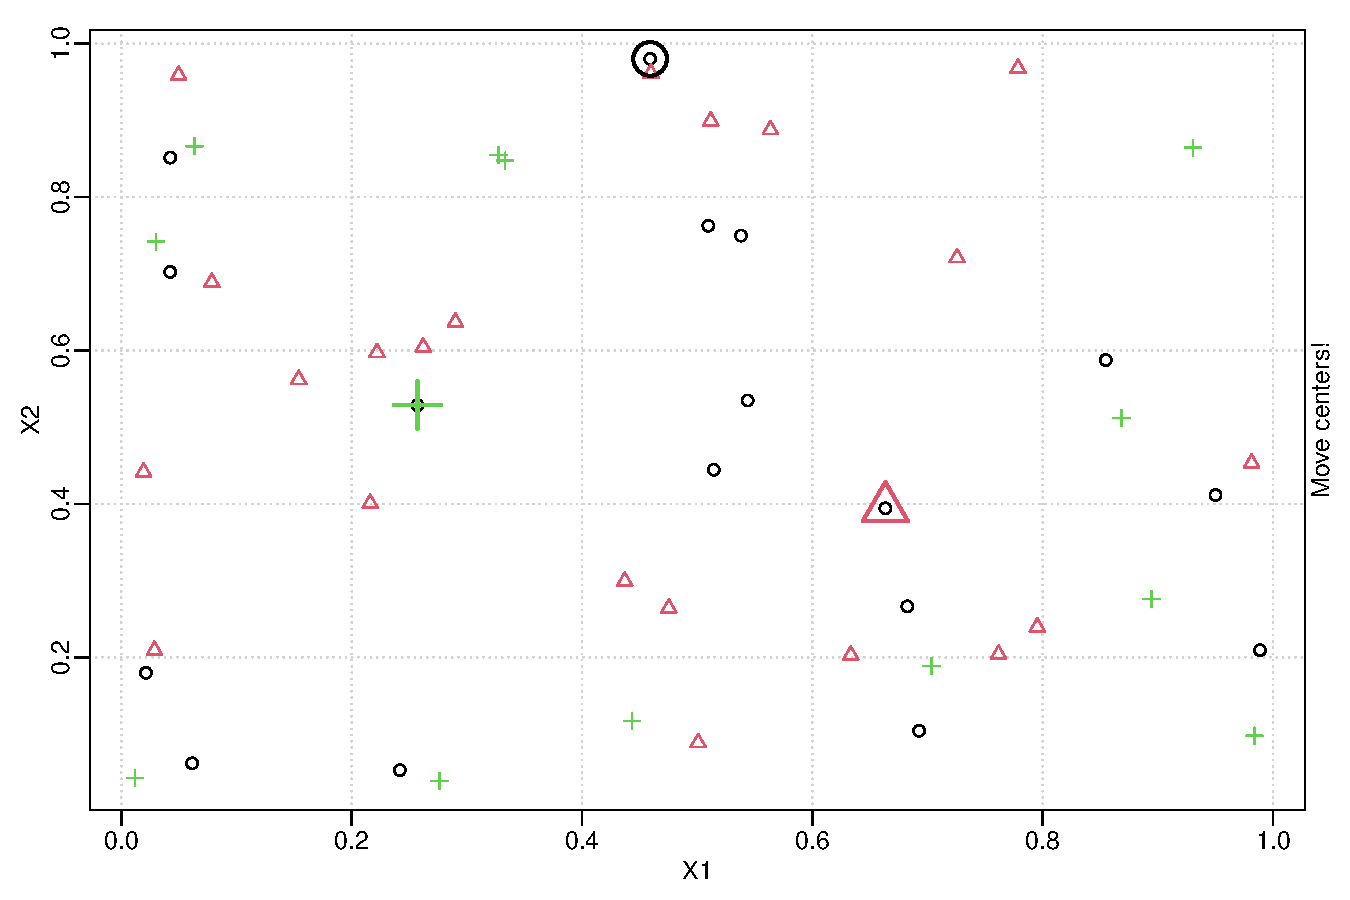
\includegraphics[width=.8\textwidth]{figures/unnamed-chunk-2-1} 

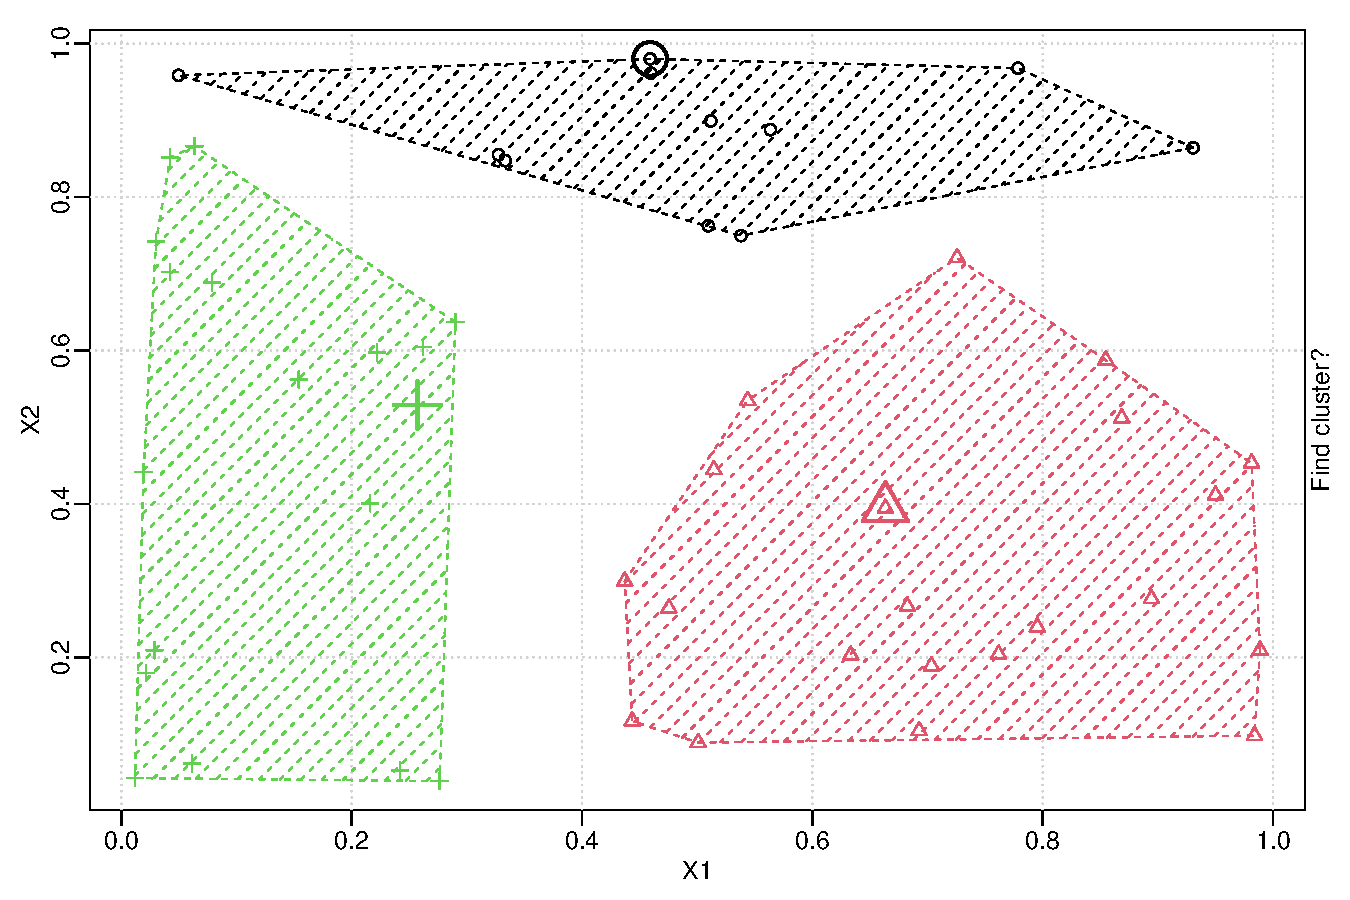
\includegraphics[width=.8\textwidth]{figures/unnamed-chunk-2-2} 

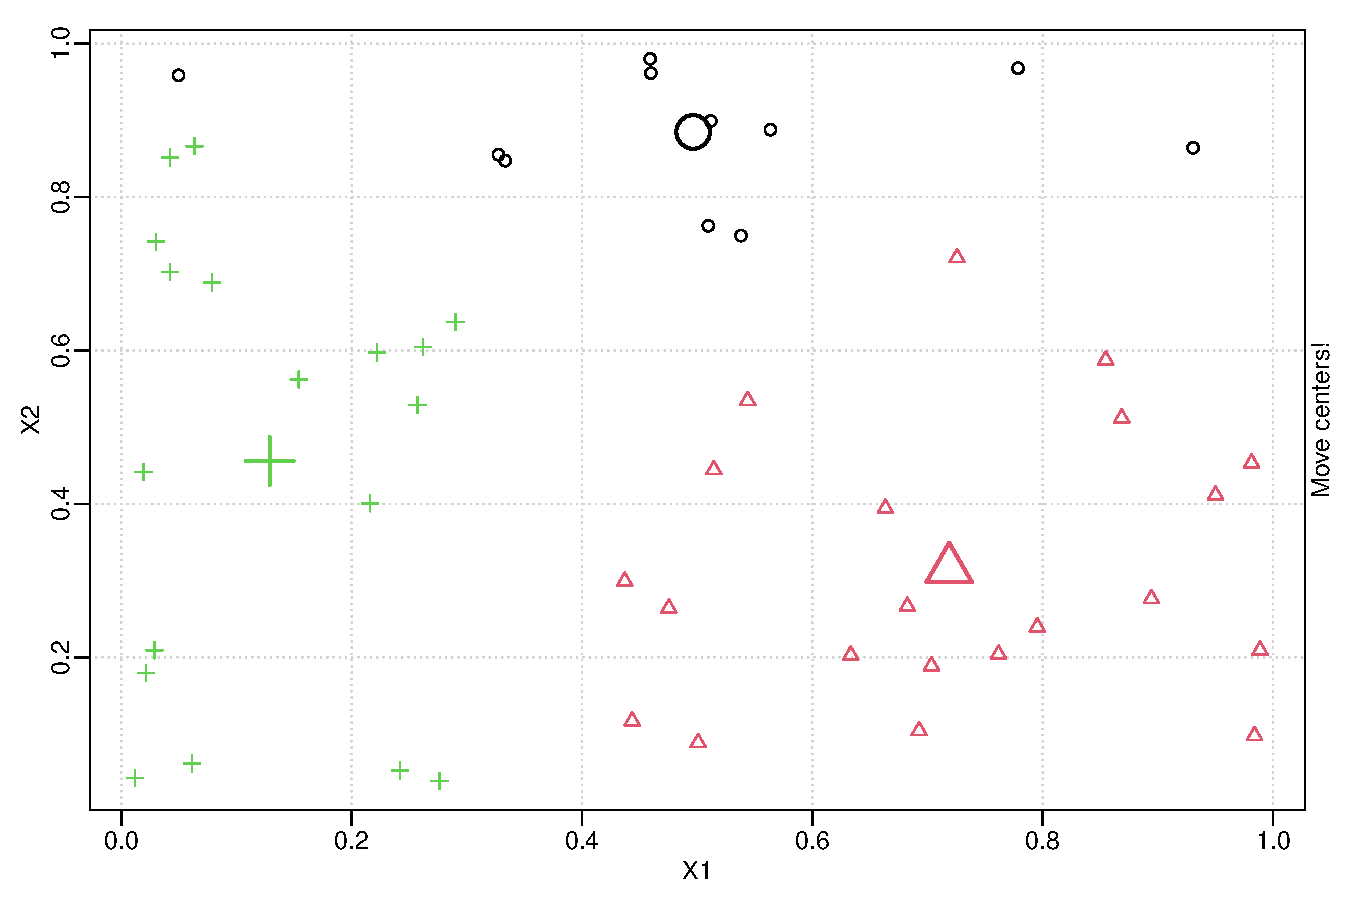
\includegraphics[width=.8\textwidth]{figures/unnamed-chunk-2-3} 

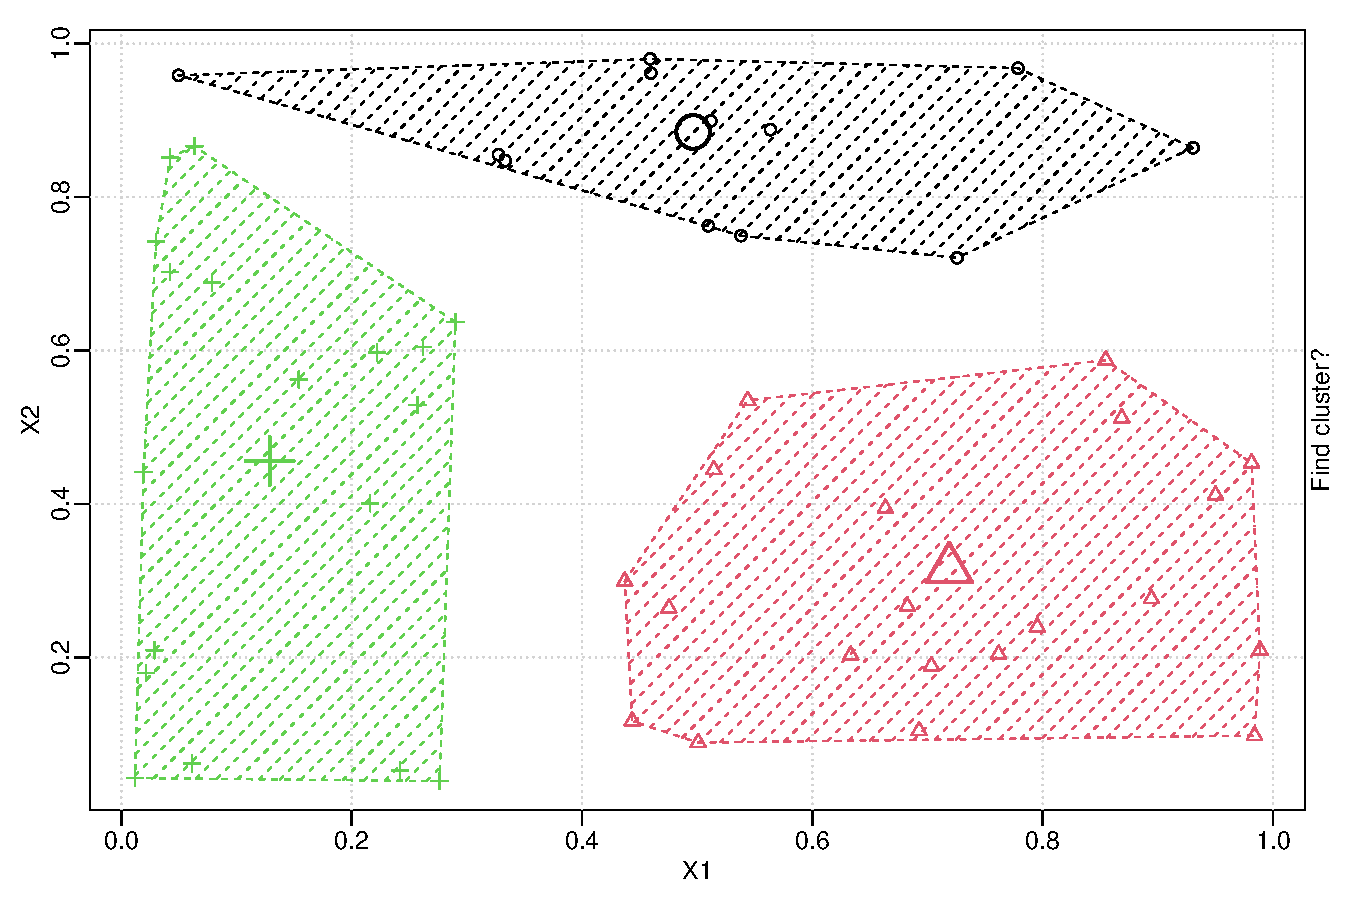
\includegraphics[width=.8\textwidth]{figures/unnamed-chunk-2-4} 

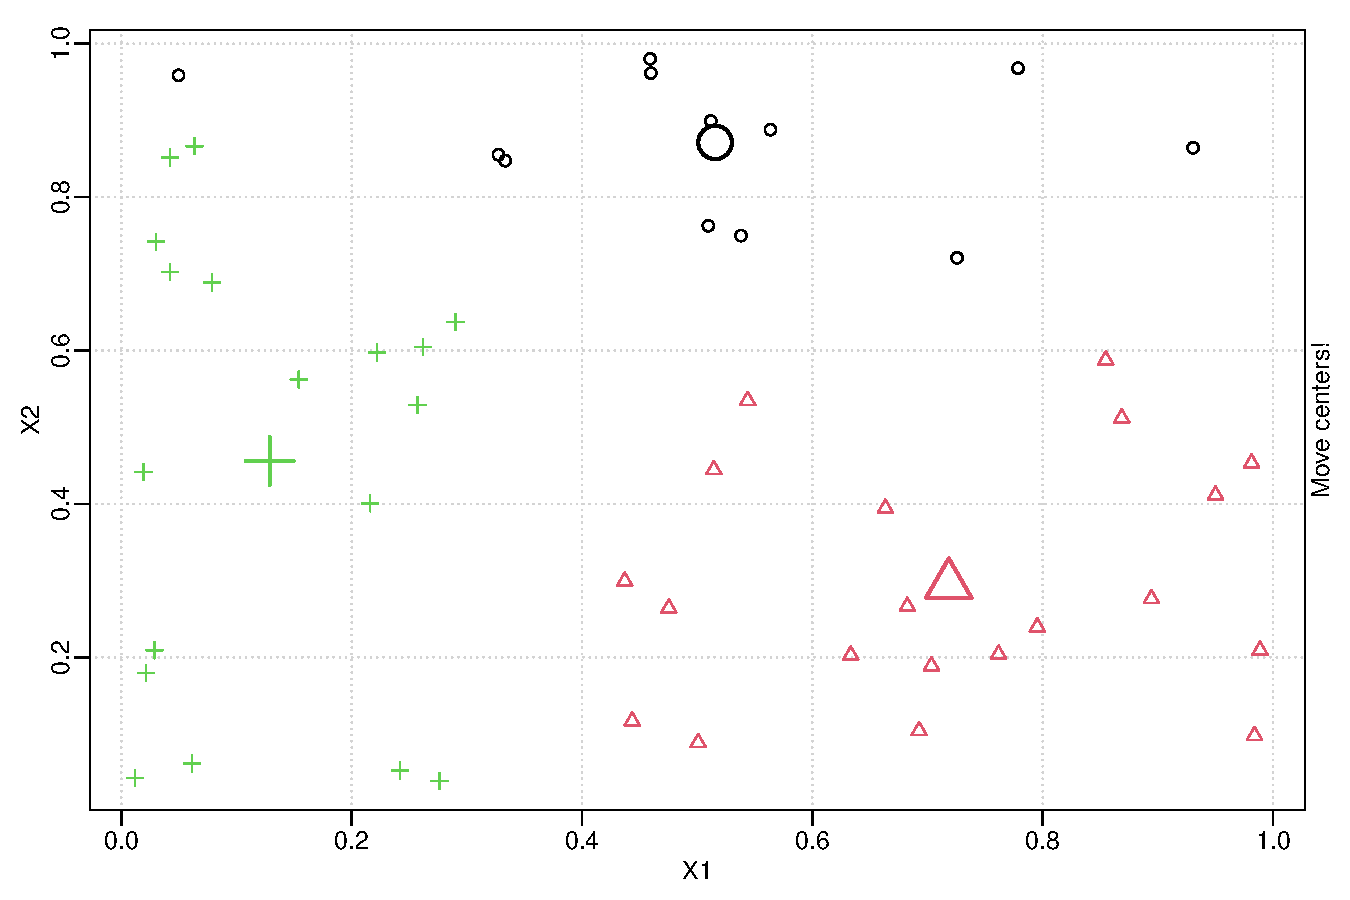
\includegraphics[width=.8\textwidth]{figures/unnamed-chunk-2-5} 

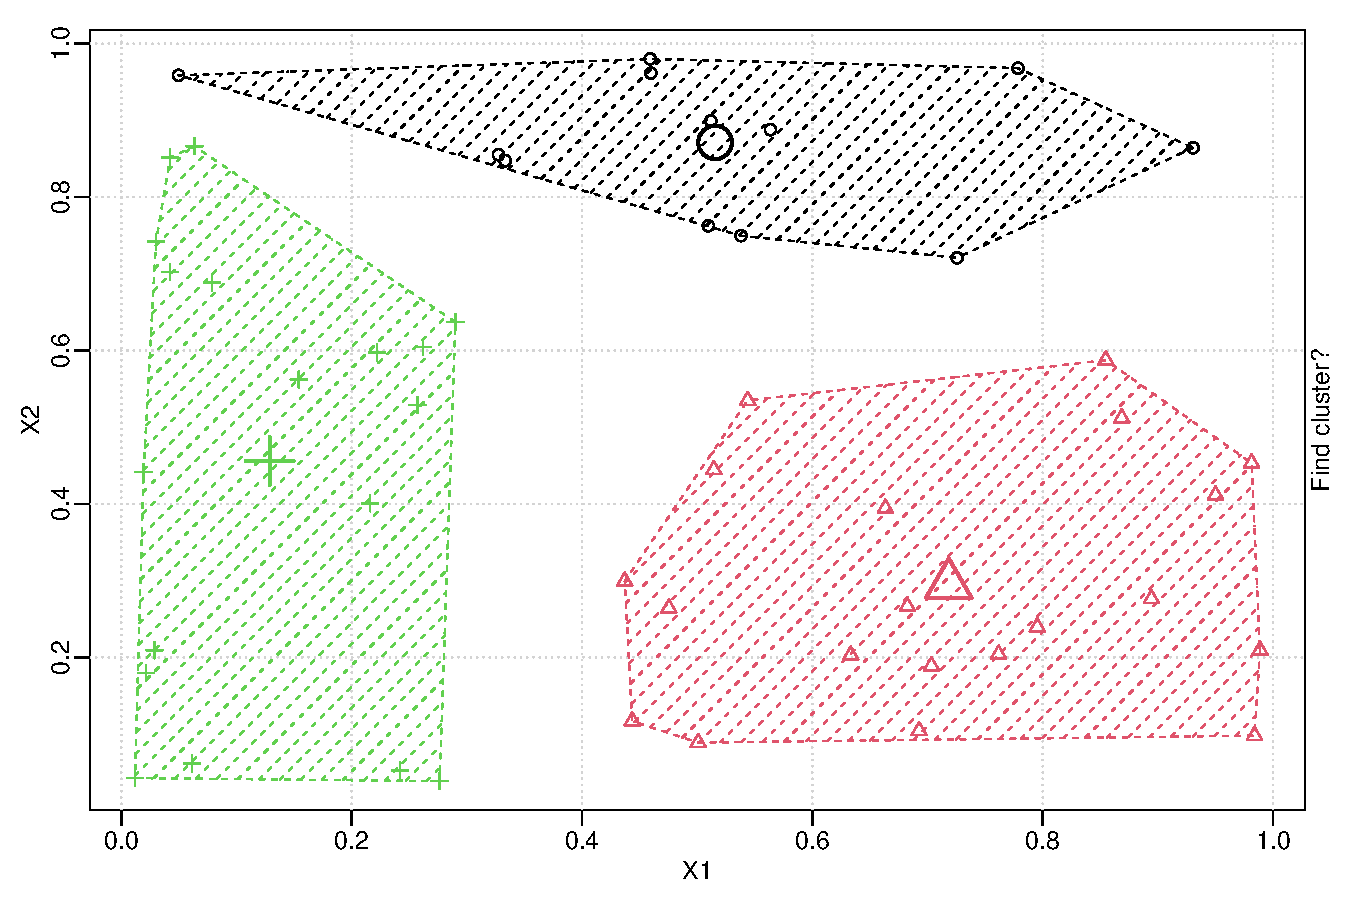
\includegraphics[width=.8\textwidth]{figures/unnamed-chunk-2-6} 

\end{knitrout}

\end{frame}

\begin{frame}
\frametitle{K-means: properties}
  
  \begin{block}{Other schemes}
    \begin{itemize}
      \item \alert{McQueen}: modify the mean each time a sample is assigned to a new cluster.
      \item \alert{Hartigan}: modify the mean by removing the considered sample, assign it to the nearby center and recompute the new mean after assignment.
    \end{itemize}
  \end{block}
  
  \begin{block}{Initialization}
    No guarantee to converge to a global optimum
    \begin{itemize}
      \item Repeat and keep the best result
      \item k-Mean++: try to take them as separated as possible.
    \end{itemize}
  \end{block}

  \begin{block}{Complexity}
     $O(n K T)$ where $T$ is the number of step in the algorithm.
  \end{block}
  
\end{frame}

\begin{frame}[fragile,allowframebreaks]
  \frametitle{K-means in \texttt{R} on uncorrected data set}

\begin{knitrout}\scriptsize
\definecolor{shadecolor}{rgb}{0.969, 0.969, 0.969}\color{fgcolor}\begin{kframe}
\begin{alltt}
\hlstd{uncor_kmeans_res} \hlkwb{<-} \hlstd{crabs} \hlopt
  \hlkwd{select}\hlstd{(}\hlopt{-}\hlstd{species,} \hlopt{-}\hlstd{sex)} \hlopt
  \hlkwd{kmeans}\hlstd{(}\hlnum{4}\hlstd{,} \hlkwc{nstart} \hlstd{=} \hlnum{10}\hlstd{)}
\hlstd{uncor_clusters} \hlkwb{<-} \hlkwd{as.factor}\hlstd{(uncor_kmeans_res}\hlopt{$}\hlstd{cluster)}
\hlstd{uncor_centers}  \hlkwb{<-} \hlkwd{as_tibble}\hlstd{(uncor_kmeans_res}\hlopt{$}\hlstd{centers)}
\hlstd{classes} \hlkwb{<-} \hlkwd{paste}\hlstd{(crabs_corrected}\hlopt{$}\hlstd{species, crabs_corrected}\hlopt{$}\hlstd{sex,} \hlkwc{sep} \hlstd{=} \hlstr{"-"}\hlstd{)}

\hlstd{crabs} \hlopt
  \hlkwd{ggplot}\hlstd{(}\hlkwd{aes}\hlstd{(}\hlkwc{x} \hlstd{= carapace_length,} \hlkwc{y} \hlstd{= carapace_width,} \hlkwc{color} \hlstd{= uncor_clusters))} \hlopt{+}
  \hlkwd{geom_point}\hlstd{(}\hlkwd{aes}\hlstd{(}\hlkwc{shape} \hlstd{= classes))} \hlopt{+}
  \hlkwd{geom_point}\hlstd{(}\hlkwc{data} \hlstd{= uncor_centers,} \hlkwc{color} \hlstd{=} \hlstr{'coral'}\hlstd{,} \hlkwc{size} \hlstd{=} \hlnum{4} \hlstd{,} \hlkwc{pch} \hlstd{=} \hlnum{21}\hlstd{)} \hlopt{+}
  \hlkwd{geom_point}\hlstd{(}\hlkwc{data} \hlstd{= uncor_centers,} \hlkwc{color} \hlstd{=} \hlstr{'coral'}\hlstd{,} \hlkwc{size} \hlstd{=} \hlnum{50}\hlstd{,} \hlkwc{alpha} \hlstd{=} \hlnum{0.2}\hlstd{)}
\end{alltt}
\end{kframe}
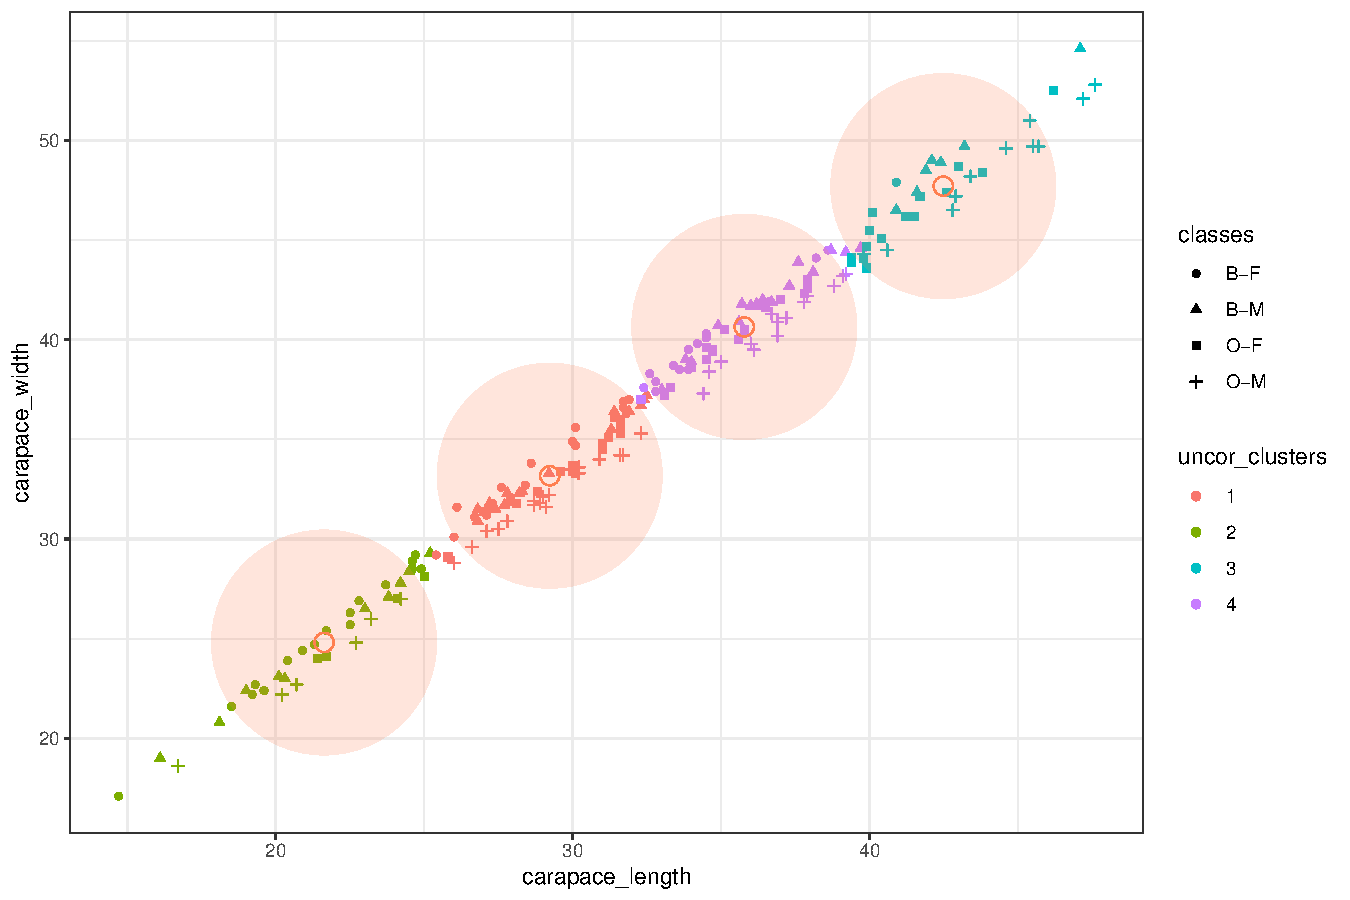
\includegraphics[width=.8\textwidth]{figures/kmeans_uncorrected_crabs-1} 

\end{knitrout}
  
\end{frame}

\begin{frame}[fragile,allowframebreaks]
  \frametitle{K-means in \texttt{R} on corrected crabs data set}
  
\begin{knitrout}\scriptsize
\definecolor{shadecolor}{rgb}{0.969, 0.969, 0.969}\color{fgcolor}\begin{kframe}
\begin{alltt}
\hlstd{kmeans_res} \hlkwb{<-} \hlstd{crabs_corrected} \hlopt
  \hlkwd{select}\hlstd{(}\hlopt{-}\hlstd{species,} \hlopt{-}\hlstd{sex)} \hlopt
  \hlkwd{kmeans}\hlstd{(}\hlnum{4}\hlstd{,} \hlkwc{nstart} \hlstd{=} \hlnum{10}\hlstd{)}
\hlstd{clusters} \hlkwb{<-} \hlkwd{as.factor}\hlstd{(kmeans_res}\hlopt{$}\hlstd{cluster)}
\hlstd{centers}  \hlkwb{<-} \hlkwd{as.tibble}\hlstd{(kmeans_res}\hlopt{$}\hlstd{centers)}
\hlstd{classes} \hlkwb{<-} \hlkwd{paste}\hlstd{(crabs_corrected}\hlopt{$}\hlstd{species, crabs_corrected}\hlopt{$}\hlstd{sex,} \hlkwc{sep} \hlstd{=} \hlstr{"-"}\hlstd{)}

\hlstd{crabs_corrected} \hlopt
  \hlkwd{ggplot}\hlstd{(}\hlkwd{aes}\hlstd{(}\hlkwc{x} \hlstd{= carapace_length,} \hlkwc{y} \hlstd{= carapace_width,} \hlkwc{color} \hlstd{= clusters))} \hlopt{+}
  \hlkwd{geom_point}\hlstd{(}\hlkwd{aes}\hlstd{(}\hlkwc{shape} \hlstd{= classes))} \hlopt{+}
  \hlkwd{geom_point}\hlstd{(}\hlkwc{data} \hlstd{= centers,} \hlkwc{color} \hlstd{=} \hlstr{'coral'}\hlstd{,} \hlkwc{size} \hlstd{=} \hlnum{4} \hlstd{,} \hlkwc{pch} \hlstd{=} \hlnum{21}\hlstd{)} \hlopt{+}
  \hlkwd{geom_point}\hlstd{(}\hlkwc{data} \hlstd{= centers,} \hlkwc{color} \hlstd{=} \hlstr{'coral'}\hlstd{,} \hlkwc{size} \hlstd{=} \hlnum{50}\hlstd{,} \hlkwc{alpha} \hlstd{=} \hlnum{0.2}\hlstd{)}
\end{alltt}
\end{kframe}
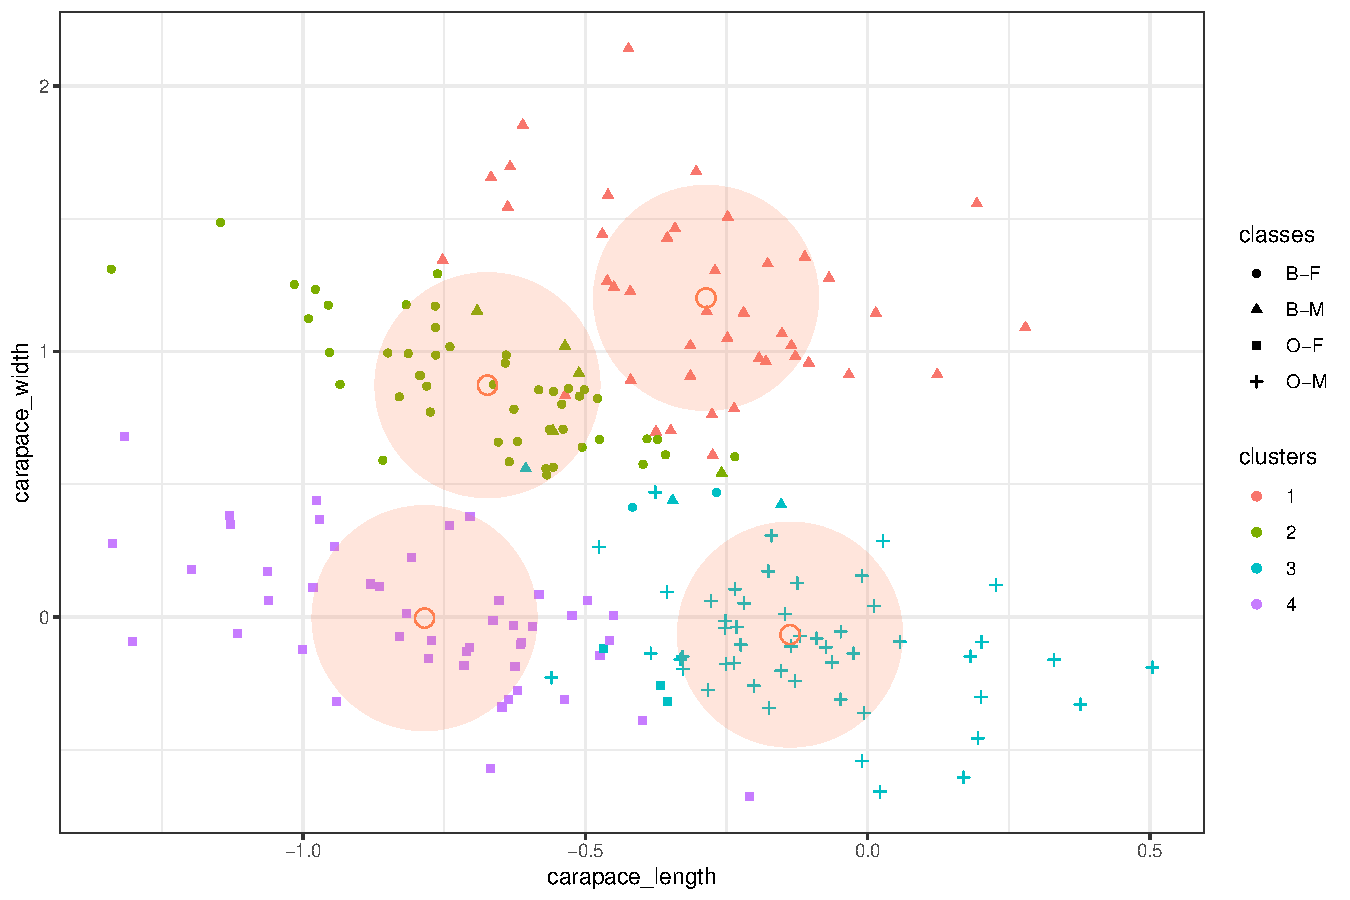
\includegraphics[width=.8\textwidth]{figures/kmeans_crabs-1} 

\end{knitrout}

\end{frame}

\begin{frame}[fragile]
  \frametitle{Clustering comparison}

\begin{knitrout}\scriptsize
\definecolor{shadecolor}{rgb}{0.969, 0.969, 0.969}\color{fgcolor}\begin{kframe}
\begin{alltt}
\hlstd{aricode}\hlopt{::}\hlkwd{ARI}\hlstd{(clusters, classes)}
\end{alltt}
\begin{verbatim}
## [1] 0.8317615
\end{verbatim}
\begin{alltt}
\hlstd{aricode}\hlopt{::}\hlkwd{ARI}\hlstd{(uncor_clusters, classes)}
\end{alltt}
\begin{verbatim}
## [1] 0.01573617
\end{verbatim}
\end{kframe}
\end{knitrout}

\begin{knitrout}\scriptsize
\definecolor{shadecolor}{rgb}{0.969, 0.969, 0.969}\color{fgcolor}\begin{kframe}
\begin{alltt}
\hlstd{knitr}\hlopt{::}\hlkwd{kable}\hlstd{(}\hlkwd{table}\hlstd{(clusters, classes),}
\hlkwc{caption} \hlstd{=} \hlstr{"Estimating structure with k-means"}\hlstd{)}
\end{alltt}
\end{kframe}\begin{table}

\caption{\label{tab:contingency_table_kmeans}Estimating structure with k-means}
\centering
\begin{tabular}[t]{r|r|r|r}
\hline
B-F & B-M & O-F & O-M\\
\hline
0 & 42 & 0 & 0\\
\hline
48 & 5 & 0 & 0\\
\hline
2 & 3 & 3 & 50\\
\hline
0 & 0 & 47 & 0\\
\hline
\end{tabular}
\end{table}


\end{knitrout}

\end{frame}


\begin{frame}[fragile,allowframebreaks]
  \frametitle{How about a "spectral" k-means?}
  \framesubtitle{PCA + k-means}

\begin{knitrout}\scriptsize
\definecolor{shadecolor}{rgb}{0.969, 0.969, 0.969}\color{fgcolor}\begin{kframe}
\begin{alltt}
\hlstd{SVD} \hlkwb{<-} \hlkwd{svd}\hlstd{(}\hlkwd{select}\hlstd{(crabs_corrected,} \hlopt{-}\hlstd{species,} \hlopt{-}\hlstd{sex))}
\hlstd{spec_crabs} \hlkwb{<-} \hlkwd{as.tibble}\hlstd{(SVD}\hlopt{$}\hlstd{u[,}\hlnum{1}\hlopt{:}\hlnum{2}\hlstd{]} \hlopt \hlkwd{diag}\hlstd{(SVD}\hlopt{$}\hlstd{d[}\hlnum{1}\hlopt{:}\hlnum{2}\hlstd{]))}
\hlstd{spec_kmeans_res} \hlkwb{<-} \hlstd{spec_crabs} \hlopt
  \hlkwd{kmeans}\hlstd{(}\hlnum{4}\hlstd{,} \hlkwc{nstart} \hlstd{=} \hlnum{10}\hlstd{)}
\hlstd{spec_clusters} \hlkwb{<-} \hlkwd{as.factor}\hlstd{(spec_kmeans_res}\hlopt{$}\hlstd{cluster)}
\hlstd{spec_centers}  \hlkwb{<-} \hlkwd{as.tibble}\hlstd{(spec_kmeans_res}\hlopt{$}\hlstd{centers)}
\hlstd{classes} \hlkwb{<-} \hlkwd{paste}\hlstd{(crabs_corrected}\hlopt{$}\hlstd{species, crabs_corrected}\hlopt{$}\hlstd{sex,} \hlkwc{sep} \hlstd{=} \hlstr{"-"}\hlstd{)}

\hlkwd{ggplot}\hlstd{(spec_crabs,} \hlkwd{aes}\hlstd{(V1, V2,} \hlkwc{color} \hlstd{= spec_clusters))} \hlopt{+}
  \hlkwd{geom_point}\hlstd{(}\hlkwd{aes}\hlstd{(}\hlkwc{shape} \hlstd{= classes))} \hlopt{+}
  \hlkwd{geom_point}\hlstd{(}\hlkwc{data} \hlstd{= spec_centers,} \hlkwc{color} \hlstd{=} \hlstr{'coral'}\hlstd{,} \hlkwc{size} \hlstd{=} \hlnum{4} \hlstd{,} \hlkwc{pch} \hlstd{=} \hlnum{21}\hlstd{)} \hlopt{+}
  \hlkwd{geom_point}\hlstd{(}\hlkwc{data} \hlstd{= spec_centers,} \hlkwc{color} \hlstd{=} \hlstr{'coral'}\hlstd{,} \hlkwc{size} \hlstd{=} \hlnum{50}\hlstd{,} \hlkwc{alpha} \hlstd{=} \hlnum{0.2}\hlstd{)}
\end{alltt}
\end{kframe}
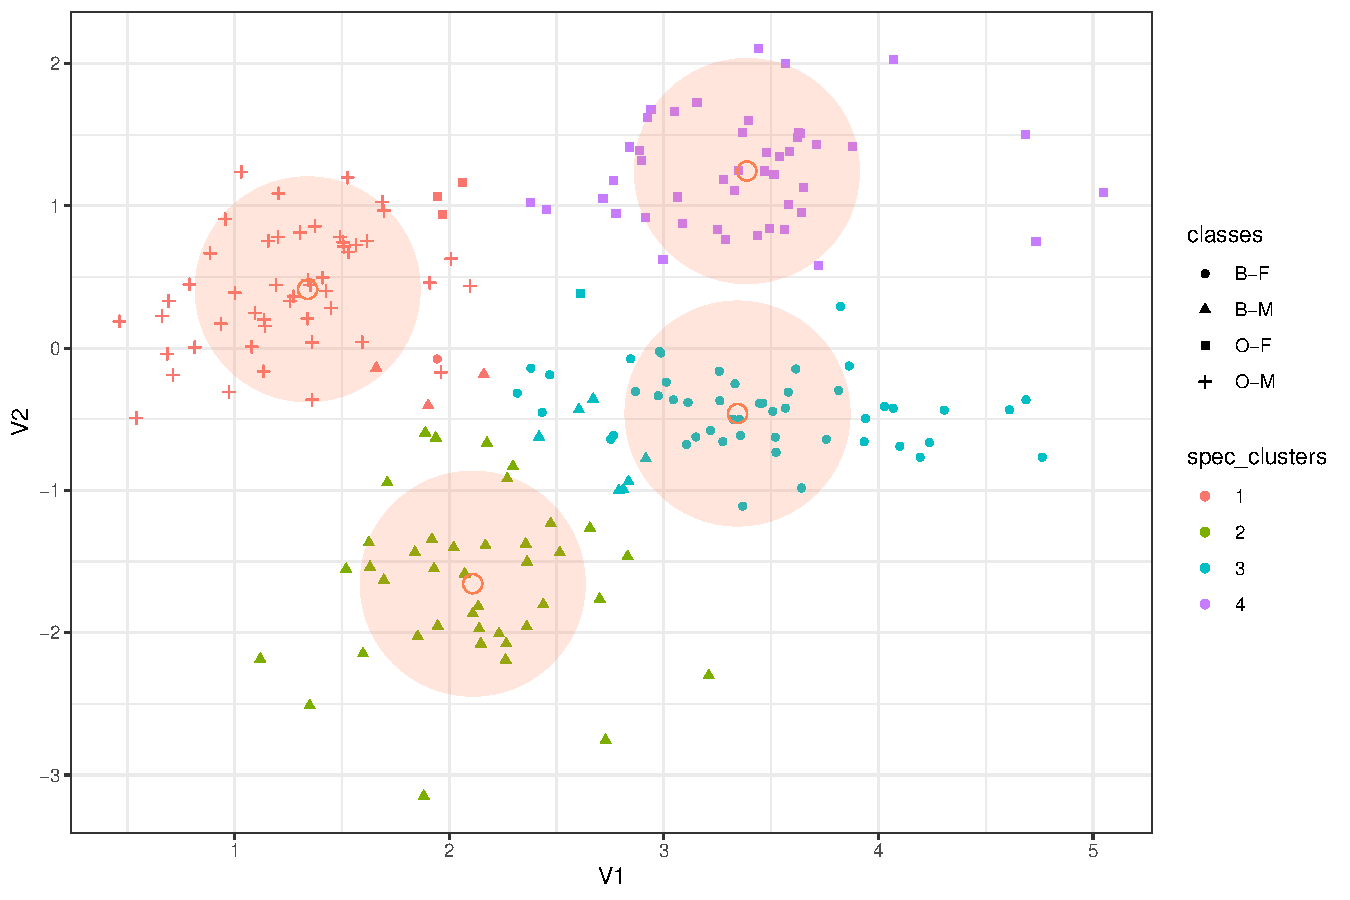
\includegraphics[width=.8\textwidth]{figures/spectral_kmeans_crabs-1} 

\end{knitrout}

\begin{knitrout}\scriptsize
\definecolor{shadecolor}{rgb}{0.969, 0.969, 0.969}\color{fgcolor}\begin{kframe}
\begin{alltt}
\hlstd{aricode}\hlopt{::}\hlkwd{ARI}\hlstd{(spec_clusters, classes)}
\end{alltt}
\begin{verbatim}
## [1] 0.8090372
\end{verbatim}
\end{kframe}
\end{knitrout}

\begin{knitrout}\scriptsize
\definecolor{shadecolor}{rgb}{0.969, 0.969, 0.969}\color{fgcolor}\begin{kframe}
\begin{alltt}
\hlstd{knitr}\hlopt{::}\hlkwd{kable}\hlstd{(}\hlkwd{table}\hlstd{(spec_clusters, classes),}
\hlkwc{caption} \hlstd{=} \hlstr{"Estimating structure with spectral k-means"}\hlstd{)}
\end{alltt}
\end{kframe}\begin{table}

\caption{\label{tab:contingency_table_spectral_kmeans}Estimating structure with spectral k-means}
\centering
\begin{tabular}[t]{r|r|r|r}
\hline
B-F & B-M & O-F & O-M\\
\hline
1 & 3 & 3 & 50\\
\hline
0 & 40 & 0 & 0\\
\hline
49 & 7 & 1 & 0\\
\hline
0 & 0 & 46 & 0\\
\hline
\end{tabular}
\end{table}


\end{knitrout}

\end{frame}

%% ==========================================================================
%% Hierarchical Clustering
%% ==========================================================================

\section{Hierarchical Agglomerative Clustering}

\begin{frame}
  \frametitle{Agglomerative Clustering: Heuristic}
    
    \begin{block}{Idea}
      \begin{enumerate}
        \item Start with small clusters (\textit{e.g.} one cluster $\equiv$ one individual)
        \item Merge the most similar clusters sequentially (and greedily)
        \item Stops when all individuals are in the same groups
      \end{enumerate}
    \end{block}

    \begin{block}{Ingredients}
      \begin{enumerate}
        \item a dissimilarity measure (distance between individuals)
        \item a merging criterion $\Delta$ (dissimilarity between clusters)
      \end{enumerate}
    \end{block}

    \begin{itemize}
      \item[+] Generates a hierarchy of clustering instead of a single partition
      \item[--] Need to select the number of cluster afterwards
    \end{itemize}
\end{frame}

\begin{frame}
  \frametitle{Agglomerative Clustering: general algorithm}

  \begin{block}{Algorithm}
    \vspace{-.25cm}
    \begin{enumerate}
      \item Start with $(\mathcal{C}_k^{(0)})= (\{ \bx_i \})$ the collection of all singletons.
      \item At step $s$, we have $n-s$ clusters $(\mathcal{C}_{k}^{(s)})$:

      \begin{itemize}
        \item Find the two most similar clusters according to a criterion $\Delta$:%%\\[-.75cm]
        \begin{align*}
          (k,\ell) = \argmin_{(k',\ell')} \Delta(\mathcal{C}_{k'}^{(s)},\mathcal{C}_{_ell'}^{(s)})
        \end{align*}
        \item Merge $\mathcal{C}_{k}^{(s)}$ and $\mathcal{C}_{\ell}^{(s)}$ into $\mathcal{C}_{k}^{(s+1)}$
        \item Update the distances between $\mathcal{C}_{k}^{(s+1)}$ and the remaining clusters
      \end{itemize}
  
      \item Repeat until there is only one cluster.
    \end{enumerate}
  \end{block}

  \vfill

  \begin{block}{Complexity}<2>
    \vspace{-.25cm}
    \begin{itemize}
      \item In general $O(n^3)$
      \item Can be reduced to $O(n^2)$ if boundering the number of merges
    \end{itemize}
  \end{block}
  
\end{frame}

\begin{frame}

  \begin{center}
    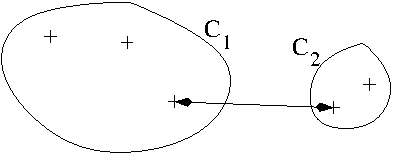
\includegraphics[width=.3\textwidth]{ex_sautmin}
    \hspace*{.1\textwidth}
    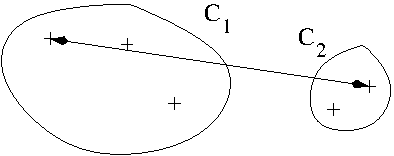
\includegraphics[width=.3\textwidth]{ex_sautmax}
  \end{center}

  \begin{block}{Merging criterion based on the distance between points}
    \begin{itemize}
      \item Single linkage (or minimum linkage):
      \begin{align*}
        \Delta(\mathcal{C}_k, \mathcal{C}_\ell) = \min_{\bx_i \in \mathcal{C}_k, \bx_j \in \mathcal{C}_\ell} d(\bx_i, \bx_j)
      \end{align*}
      \item Complete linkage (or maximum linkage):
      \begin{align*}
        \Delta(\mathcal{C}_k, \mathcal{C}_\ell) = \max_{\bx_i \in \mathcal{C}_k} \max_{\bx_j \in \mathcal{C}_\ell}d(\bx_i, \bx_j)
    \end{align*}
    \item Average linkage (or group linkage):
      \begin{align*}
        \Delta(\mathcal{C}_k, \mathcal{C}_\ell) = \frac{1}{|\mathcal{C}_k||\mathcal{C}_\ell|} \sum_{\bx_i \in \mathcal{C}_k}\sum_{\bx_ \in\mathcal{C}_\ell} d(\bx_i, \bx_j)
      \end{align*}
    \end{itemize}
  \end{block}

\end{frame}

\begin{frame}
  \frametitle{Ward's criteria}
  
  \begin{block}{Merging criterion based on distance to the mean}
    Ward's criterion:
    \begin{align*}
      \Delta(\mathcal{C}_k, \mathcal{C}_\ell) 
        & = \sum_{\bx_i \in \mathcal{C}_k} \left( d^2(\bx_i, \bmu_{\mathcal{C}_k \cup \mathcal{C}_\ell} ) - d^2(\bx_i, \bmu_{\mathcal{C}_k}) \right) \\
        & \quad + \sum_{\bx_j \in \mathcal{C}_\ell} \left( d^2(\bx_j, \bmu_{\mathcal{C}_j \cup \mathcal{C}_\ell} ) - d^2(\bx_j, \bmu_{\mathcal{C}_\ell}) \right)
      \end{align*}
    \end{block}

    \begin{block}{Euclidean case}
       If $d$ is the Euclidean distance, then
      \begin{align*}
        \Delta(\mathcal{C}_k, \mathcal{C}_\ell) = \frac{2|\mathcal{C}_k||\mathcal{C}_\ell|}{|\mathcal{C}_k|+|\mathcal{C}_\ell|}d^2(\bmu_{\mathcal{C}_k}, \bmu_{\mathcal{C}_\ell})
      \end{align*}
    \end{block}

\end{frame}

\begin{frame}
  \frametitle{Ward's criteria: details}
  
  Recall that the inertia measures the homogenity of the size-K clustering
  \begin{equation*}
    I_W = \sum_{k=1}^K \sum_{\bx_i \in \mathcal{C}_k} \| \bx_i - \bmu_{\mathcal{C}_k}  \|_2^2, \quad I_B = \sum_{k=1}^K n_k \| \bmu_k - \bmu  \|_2^2
  \end{equation*}
  
  \onslide<2->{
  Consider the following two partitions 
  \begin{itemize}
    \item  $\mathcal{P} = (\mathcal{C}_1, \dots,\mathcal{C}_K)$ at one level of the hierarchy $\Omega$
    \item  $\mathcal{P}'$ is $\mathcal{P}$ once $\mathcal{C}_k, \mathcal{C}_\ell$ merged
  \end{itemize}
  Then
  \begin{equation*}
    I_W(\mathcal{P}') - I_W(\mathcal{P}) = \frac{|\mathcal{C}_k||\mathcal{C}_\ell|}{|\mathcal{C}_k|+|\mathcal{C}_\ell|}d^2(\bmu_{\mathcal{C}_k}, \bmu_{\mathcal{C}_\ell}) = \frac{1}{2} \Delta(\mathcal{C}_k, \mathcal{C}_\ell).
  \end{equation*}
  }

  \onslide<3>{
  \begin{itemize}
    \item[$\rightsquigarrow$] At each step, Ward limits the loss (increase) of the intra (inter) class variance
    \item[$\rightsquigarrow$] Defines an indexed hierarchy (height of the dendrogram)
    \item[$\rightsquigarrow$] Same criteria as in the K-means algorithm
  \end{itemize}
  }

\end{frame}

\begin{frame}[fragile]
  \frametitle{Ward agglomerative clustering in \texttt{R}}
  
\begin{knitrout}\scriptsize
\definecolor{shadecolor}{rgb}{0.969, 0.969, 0.969}\color{fgcolor}\begin{kframe}
\begin{alltt}
\hlstd{Ward} \hlkwb{<-} \hlstd{crabs_corrected} \hlopt
  \hlkwd{select}\hlstd{(}\hlopt{-}\hlstd{sex,} \hlopt{-}\hlstd{species)} \hlopt
  \hlkwd{dist}\hlstd{(}\hlkwc{method} \hlstd{=} \hlstr{"euclidean"}\hlstd{)} \hlopt
  \hlkwd{hclust}\hlstd{(}\hlkwc{method} \hlstd{=} \hlstr{"ward.D2"}\hlstd{)}
\hlkwd{plot}\hlstd{(Ward)}
\end{alltt}
\end{kframe}
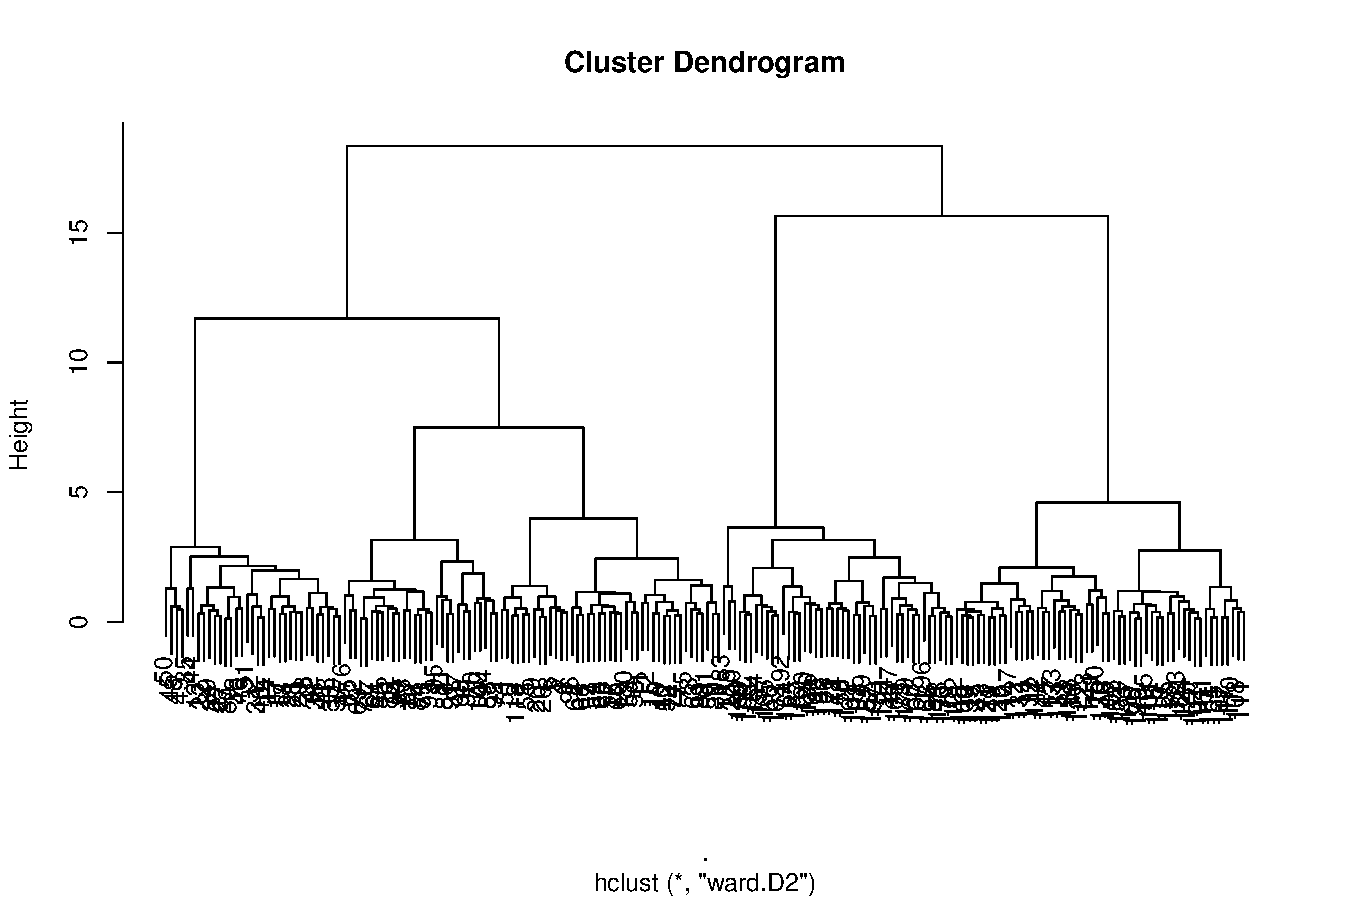
\includegraphics[width=.8\textwidth]{figures/Ward-1} 

\end{knitrout}

\end{frame}

\begin{frame}[fragile,allowframebreaks]
  \frametitle{Ward agglomerative clustering in \texttt{R}: comparison}

Compare with out reference classification and k-means
\begin{knitrout}\scriptsize
\definecolor{shadecolor}{rgb}{0.969, 0.969, 0.969}\color{fgcolor}\begin{kframe}
\begin{alltt}
\hlstd{aricode}\hlopt{::}\hlkwd{ARI}\hlstd{(}\hlkwd{cutree}\hlstd{(Ward,} \hlnum{4}\hlstd{), classes)}
\end{alltt}
\begin{verbatim}
## [1] 0.7071894
\end{verbatim}
\begin{alltt}
\hlstd{aricode}\hlopt{::}\hlkwd{ARI}\hlstd{(}\hlkwd{cutree}\hlstd{(Ward,} \hlnum{4}\hlstd{), clusters)}
\end{alltt}
\begin{verbatim}
## [1] 0.7538279
\end{verbatim}
\end{kframe}
\end{knitrout}

\begin{knitrout}\scriptsize
\definecolor{shadecolor}{rgb}{0.969, 0.969, 0.969}\color{fgcolor}\begin{kframe}
\begin{alltt}
\hlstd{knitr}\hlopt{::}\hlkwd{kable}\hlstd{(}\hlkwd{table}\hlstd{(clusters,} \hlkwd{cutree}\hlstd{(Ward,}\hlnum{4}\hlstd{)),}
\hlkwc{caption} \hlstd{=} \hlstr{"k-means vs Ward"}\hlstd{)}
\end{alltt}
\end{kframe}\begin{table}

\caption{\label{tab:contingency_table_kmeans_vs_ward}k-means vs Ward}
\centering
\begin{tabular}[t]{r|r|r|r}
\hline
1 & 2 & 3 & 4\\
\hline
9 & 33 & 0 & 0\\
\hline
53 & 0 & 0 & 0\\
\hline
6 & 0 & 52 & 0\\
\hline
2 & 0 & 2 & 43\\
\hline
\end{tabular}
\end{table}


\end{knitrout}


Optimize over a range of values
\begin{knitrout}\scriptsize
\definecolor{shadecolor}{rgb}{0.969, 0.969, 0.969}\color{fgcolor}\begin{kframe}
\begin{alltt}
\hlstd{Ward} \hlopt  \hlkwd{cutree}\hlstd{(}\hlkwc{k} \hlstd{=} \hlnum{1}\hlopt{:}\hlnum{10}\hlstd{)} \hlopt  \hlkwd{as.data.frame}\hlstd{()} \hlopt \hlkwd{as.list}\hlstd{()} \hlopt
  \hlkwd{sapply}\hlstd{(aricode}\hlopt{::}\hlstd{ARI, classes)} \hlopt \hlkwd{plot}\hlstd{(}\hlkwc{type} \hlstd{=} \hlstr{"l"}\hlstd{)}
\end{alltt}
\end{kframe}
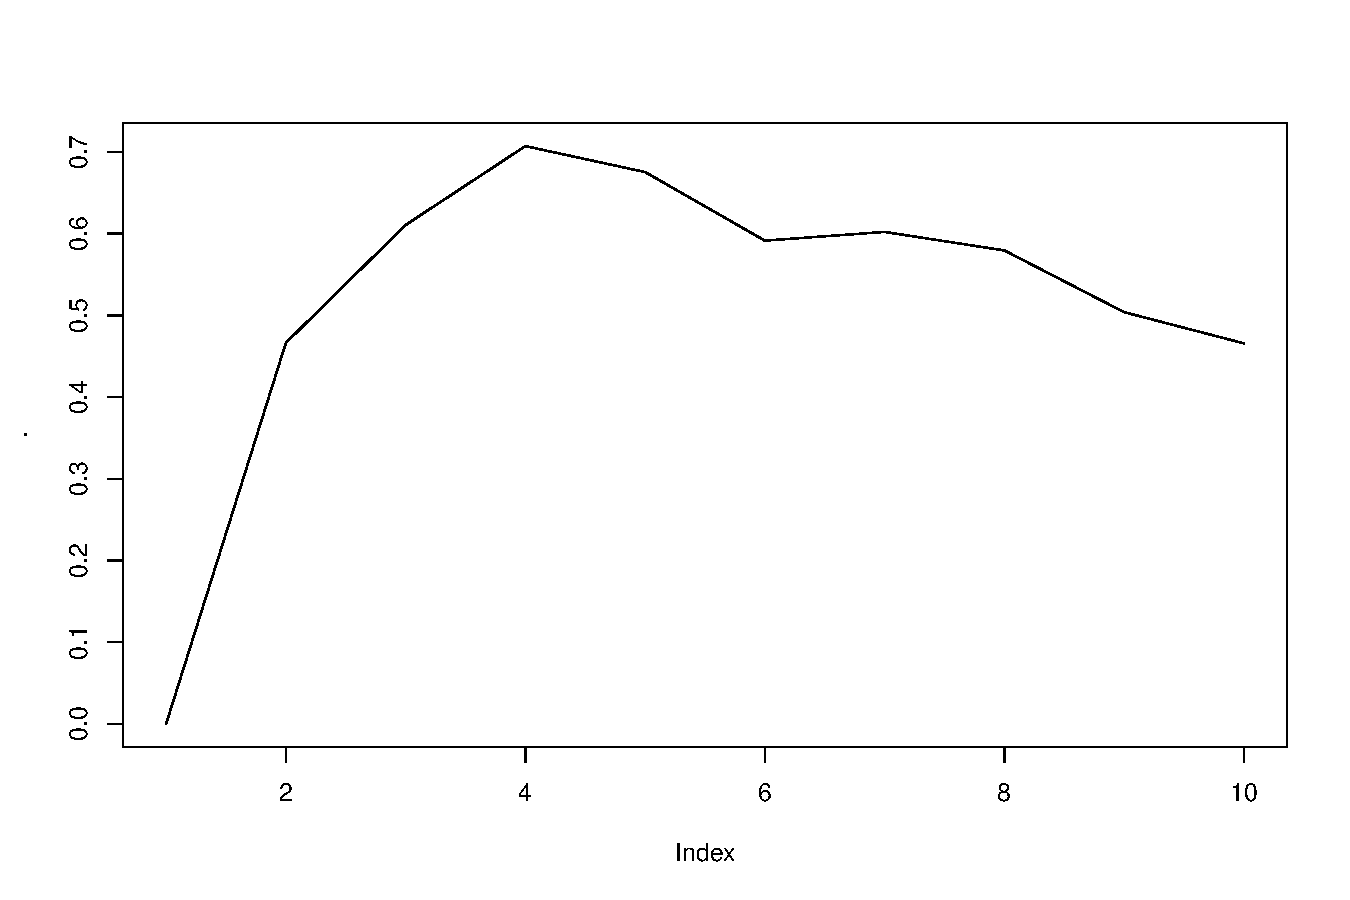
\includegraphics[width=.8\textwidth]{figures/Ward_ARIs-1} 

\end{knitrout}

Look at Ward intra-class variance
\begin{knitrout}\scriptsize
\definecolor{shadecolor}{rgb}{0.969, 0.969, 0.969}\color{fgcolor}\begin{kframe}
\begin{alltt}
\hlkwd{plot}\hlstd{(}\hlkwd{rev}\hlstd{(Ward}\hlopt{$}\hlstd{height)[}\hlnum{1}\hlopt{:}\hlnum{20}\hlstd{],} \hlkwc{xlab} \hlstd{=} \hlstr{"number of clusters"}\hlstd{,} \hlkwc{ylab} \hlstd{=} \hlstr{"height"}\hlstd{)}
\end{alltt}
\end{kframe}
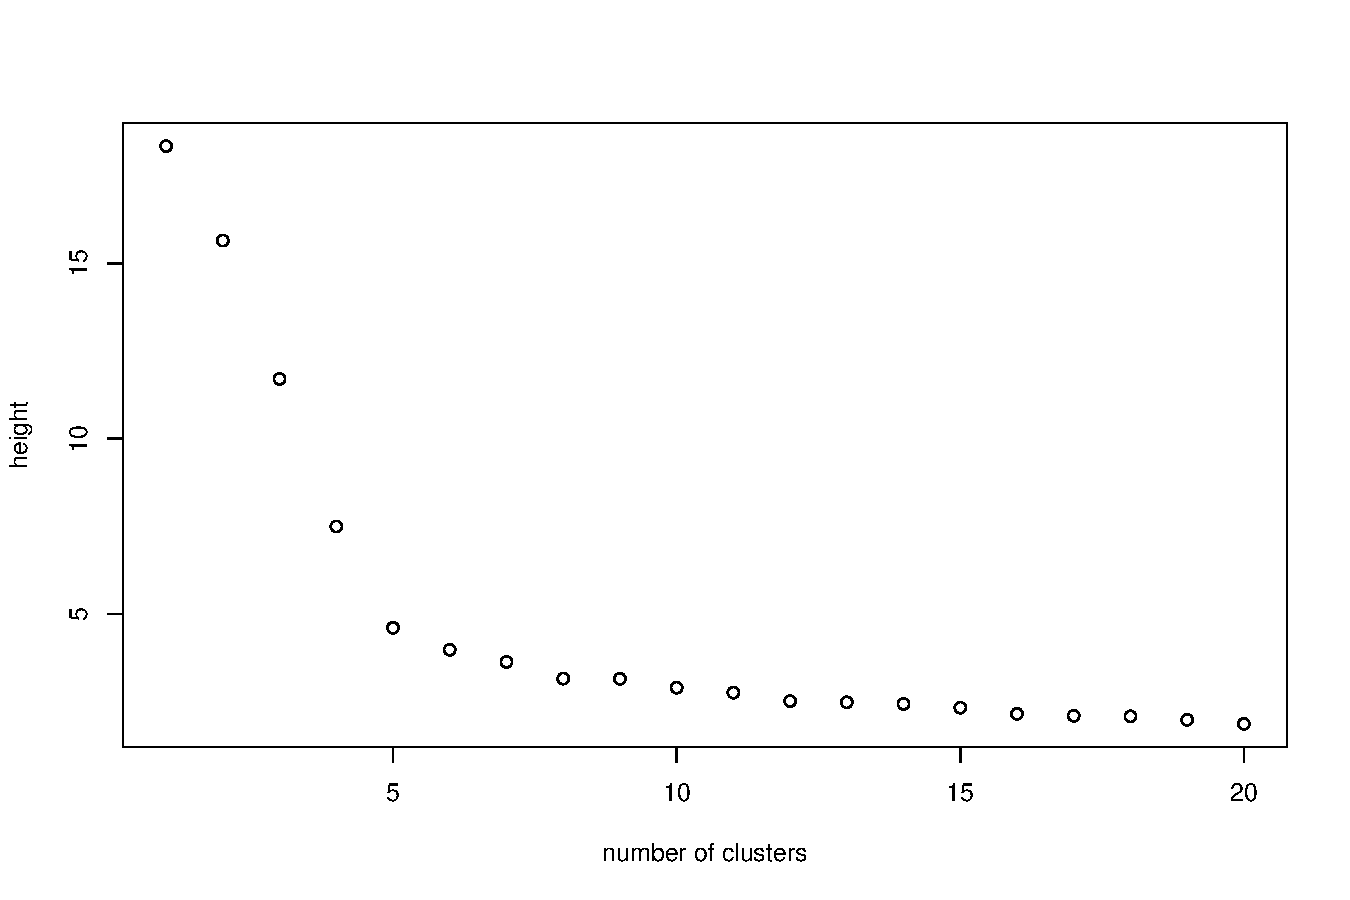
\includegraphics[width=.8\textwidth]{figures/criteria-1} 

\end{knitrout}

\end{frame}

\begin{frame}[fragile,allowframebreaks]
  \frametitle{Ward agglomerative clustering in \texttt{R}: projection}

\begin{knitrout}\scriptsize
\definecolor{shadecolor}{rgb}{0.969, 0.969, 0.969}\color{fgcolor}\begin{kframe}
\begin{alltt}
\hlstd{clusters_ward} \hlkwb{<-} \hlkwd{as.factor}\hlstd{(}\hlkwd{cutree}\hlstd{(Ward,} \hlnum{4}\hlstd{))}
\hlstd{centers_ward}  \hlkwb{<-} \hlkwd{select}\hlstd{(crabs_corrected,} \hlopt{-}\hlstd{sex,} \hlopt{-}\hlstd{species)} \hlopt
  \hlkwd{aggregate}\hlstd{(}\hlkwd{list}\hlstd{(}\hlkwd{cutree}\hlstd{(Ward,} \hlnum{4}\hlstd{)), mean)} \hlopt \hlkwd{as_tibble}\hlstd{()} \hlopt \hlkwd{select}\hlstd{(}\hlopt{-}\hlstd{Group.1)}

\hlstd{crabs_corrected} \hlopt
  \hlkwd{ggplot}\hlstd{(}\hlkwd{aes}\hlstd{(}\hlkwc{x} \hlstd{= carapace_length,} \hlkwc{y} \hlstd{= carapace_width,} \hlkwc{color} \hlstd{= clusters_ward))} \hlopt{+}
  \hlkwd{geom_point}\hlstd{(}\hlkwd{aes}\hlstd{(}\hlkwc{shape} \hlstd{= classes))} \hlopt{+}
  \hlkwd{geom_point}\hlstd{(}\hlkwc{data} \hlstd{= centers_ward,} \hlkwc{color} \hlstd{=} \hlstr{'coral'}\hlstd{,} \hlkwc{size} \hlstd{=} \hlnum{4} \hlstd{,} \hlkwc{pch} \hlstd{=} \hlnum{21}\hlstd{)} \hlopt{+}
  \hlkwd{geom_point}\hlstd{(}\hlkwc{data} \hlstd{= centers_ward,} \hlkwc{color} \hlstd{=} \hlstr{'coral'}\hlstd{,} \hlkwc{size} \hlstd{=} \hlnum{50}\hlstd{,} \hlkwc{alpha} \hlstd{=} \hlnum{0.2}\hlstd{)}
\end{alltt}
\end{kframe}
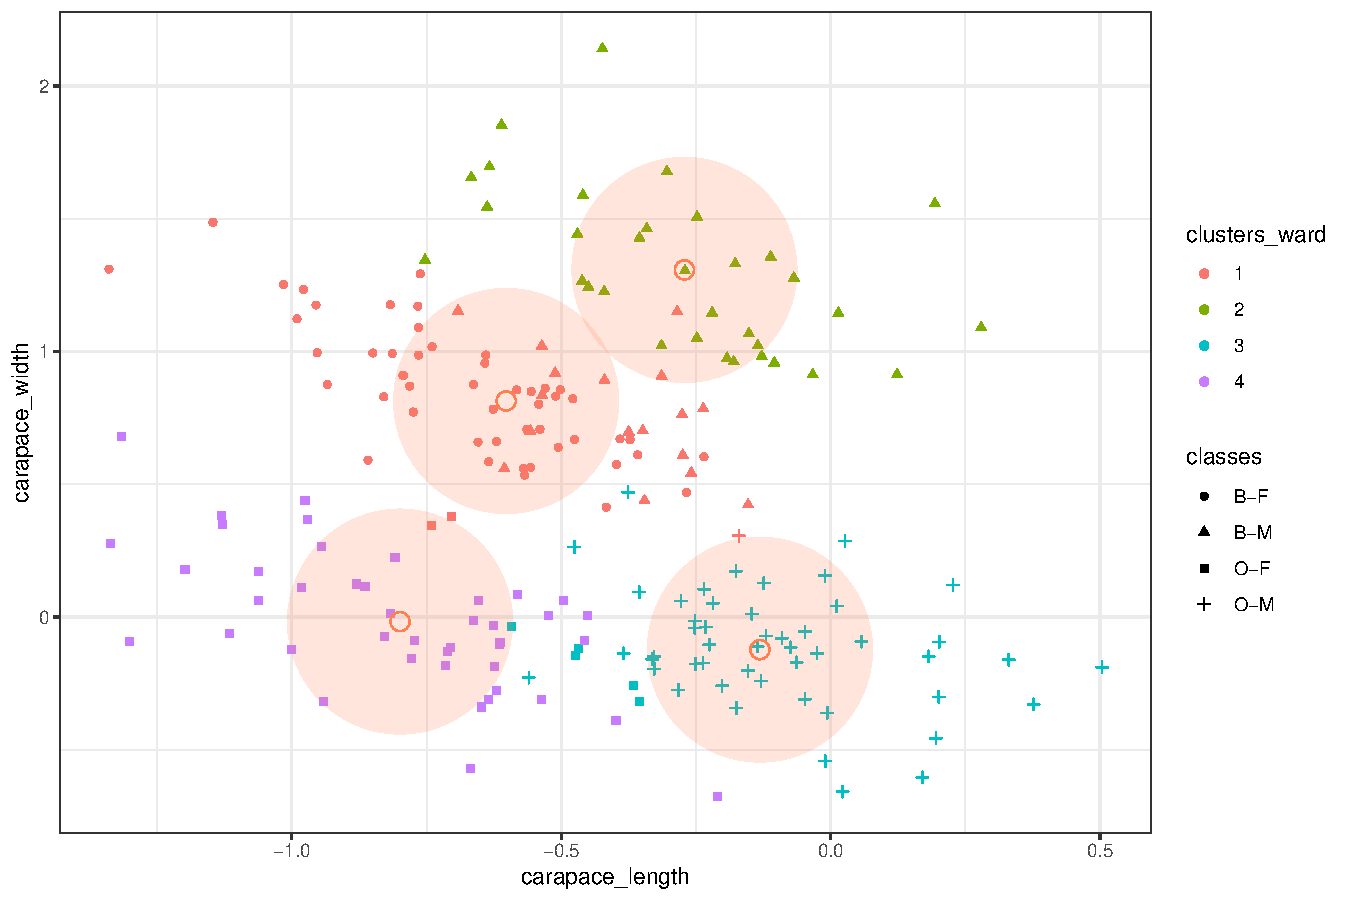
\includegraphics[width=.8\textwidth]{figures/Ward_projection-1} 

\end{knitrout}
\end{frame}

% \begin{frame}[fragile]
%   \frametitle{Reordered correlation matrix between individuals}
%   
% <<Ward corrplot>>=
% C <- cor(t(select(crabs_corrected, -sex, -species)))
% C <- C[order(clusters_ward),order(clusters_ward)]
%   corrplot(C, method = "color", tl.pos = "n")
% @
%   
% 
% \end{frame}

%% ==========================================================================
%% Spectral Clustering
%% ==========================================================================

\section{Spectral Clustering}

\begin{frame} 
  \frametitle{References}

    \begin{thebibliography}{99}
      \setbeamertemplate{bibliography item}[book]

    \bibitem{DS}{DS} David Sontag's Lecture
    \newblock \url{http://people.csail.mit.edu/dsontag/courses/ml13/slides/lecture16.pdf}
    
    \bibitem[VLB]{VLB} A Tutorial on Spectral Clustering, 
    \newblock \textcolor{black}{Ulrike von Luxburg}

    \end{thebibliography}

\end{frame}

\begin{frame}
  \frametitle{Spectral Clustering}
  
  \begin{block}{Principle: graph-based transformation prior to clustering} 
    \begin{enumerate}
      \item Build a similarity with a weighted graph of the data 
      \item Use the spectral property of this similarity (\rsa kernel)
      \item Apply clustering (e.g., k-means) to the projected data 
    \end{enumerate}
  \end{block}

  \begin{figure}[ht]
    \centering
    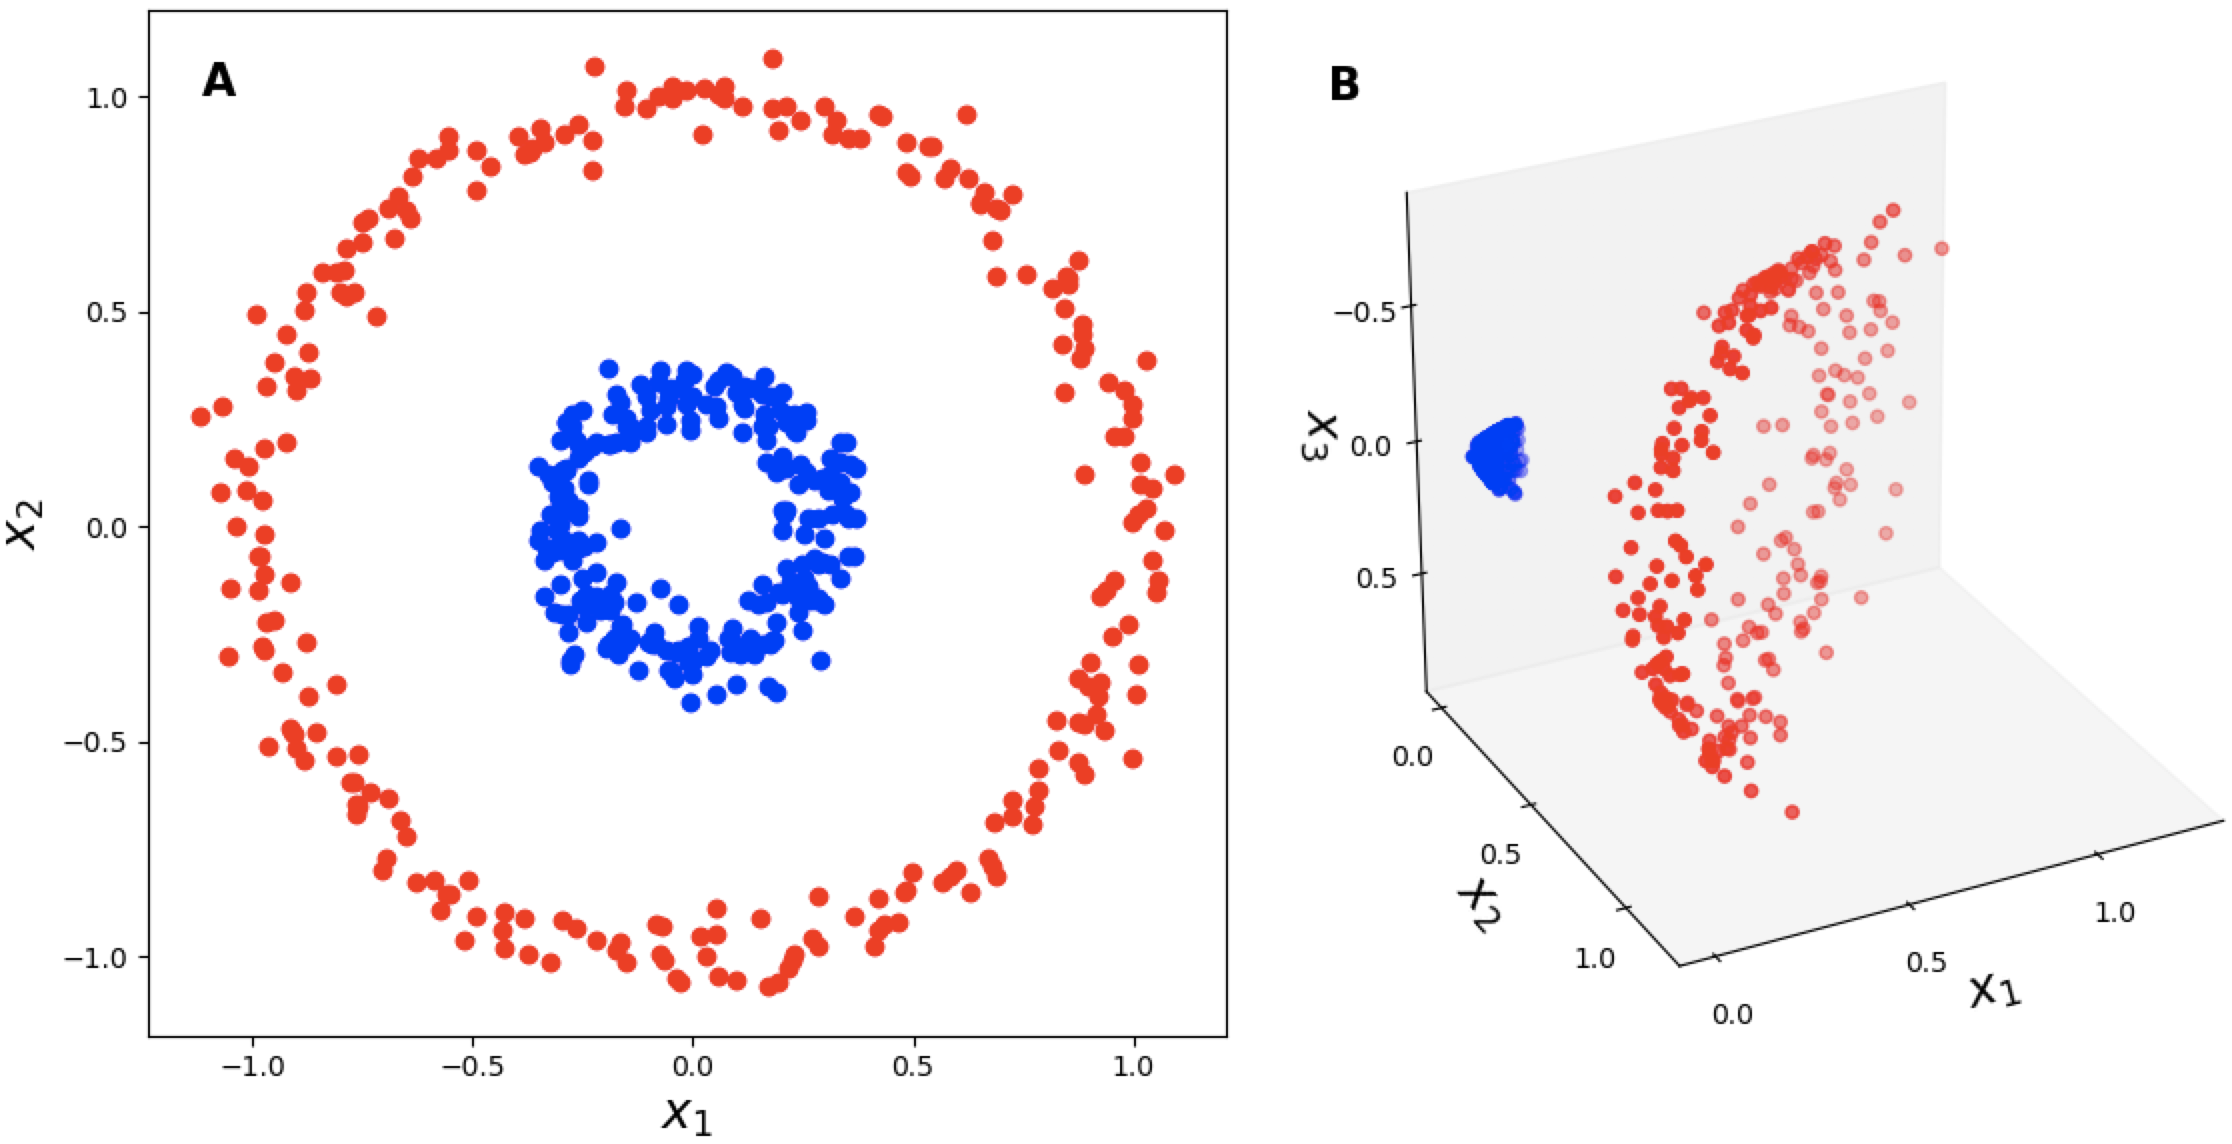
\includegraphics[height=4cm]{figures/kernel_trick2}
    \caption{Performing clustering after transformation + dimension reduction of the data }
  \end{figure}

\end{frame}

\begin{frame}
  \frametitle{Creating the graph}
  
  \begin{block}{Many choices}    
    \begin{itemize}
      \item K-nearest neighbor graph
      \item any distance-based similarity (fully connected graph)
      \item any kernel-based similarity (e.g., Gaussian kernel)
    \end{itemize}
  \end{block}

  The connectivity of $\clG = (\clV,\clE)$ is captured by the (weighted) adjacency matrix $\bA$:
    \[
      (\bA)_{ij} = \begin{cases}
      w_{ij} > 0  & \text{ if } i \sim j,\\
      0  & \text{otherwise}.
      \end{cases}
    \]

  \begin{proposition}
    The degrees of $\clG$ are then simply obtained as the row-wise and/or column-wise sums of $\bA$.
  \end{proposition}

\end{frame}

\begin{frame}
  \frametitle{Incidence matrix}

  \begin{definition}[Incidence matrix]
    The connectivity of $\clG = (\clV,\clE)$ is captured by the $|\clV|\times |\clE|$ matrix $\bB$:
    \[
      (\bB)_{ij} = \begin{cases}
      \sqrt{w_{ij}}  & \text{ if $i$ is incident to edge $j$},\\
      0  & \text{otherwise}.
      \end{cases}
    \]
  \end{definition}

  \begin{proposition}[Relationship]
    Let $\tilde\bB$ be a modified \alert{signed} version of $\bB$ where $\tilde{\! B}_{ij}= +/-\sqrt{w_{ij}}$ if $i$ is incident to $j$ as tail/head. Then
    \[
      \tilde \bB \tilde \bB^\intercal = \bD - \bA,
    \]
    where $\bD = \diag(\set{d_i, i\in\clV})$ is the diagonal matrix of degrees. 
  \end{proposition}

\end{frame}

\begin{frame}
  \frametitle{Graph Laplacian}

  \begin{definition}[(Un-normalized) Laplacian]
    The Laplacian matrix $\bL$, resulting from the modified incidence matrix $\tilde\bB$ $\tilde{\! B}_{ij}= 1/-1$ if $i$ is incident to $j$ as tail/head, is defined by 
    \[
      \bL = \tilde \bB \tilde \bB^\intercal = \bD - \bA,
    \]
    where $\bD = \diag(d_i, i\in\clV)$ is the diagonal matrix of degrees. 
  \end{definition}

  \begin{block}{Remark}
    \begin{itemize}
    \item $\bL$ is called the graph Laplacian (by analogy to continuous Laplacian).
    \item Spectrum of $\bL$ has much to say about the structure of the graph $\clG$.
    \end{itemize}
  \end{block}

\end{frame}

\begin{frame}
  \frametitle{Graph Laplacian: spectrum}

  \begin{proposition}[Spectrum of $\bL$]
    The $n\times n$ matrix $\bL$ has the following properties:
    \[
      \bx^\top \bL \bx = \frac{1}{2} \sum_{i,j} A_{ij} (x_i - x_j)^2, \quad \forall \bx\in\Rset^n .
    \]
    \vspace{-.25cm}
    \begin{itemize}
      \item $\bL$ is a symmetric, positive semi-definite matrix,
      \item  the smallest eigenvalue is $0$ with associated eigenvector $\mathbf{1}$.
      \item $\bL$ has $n$ positive eigenvalues $0=\lambda_1<\dots <\lambda_n$. 
    \end{itemize}  
  \end{proposition}

  \begin{corollary}[Spectrum and Graph]
    \vspace{-.25cm}
    \begin{itemize}
      \item The multiplicity of the first eigen value ($0$) of $\bL$ determines the number of connected components in the graph.
      \item The larger the second non trivial eigenvalue, the higher the connectivity of $\clG$.
    \end{itemize}  
  \end{corollary}

\end{frame}

\begin{frame}[fragile,allowframebreaks]
  \frametitle{Crabs: Fielder vector and eigenvalue}

\begin{knitrout}\scriptsize
\definecolor{shadecolor}{rgb}{0.969, 0.969, 0.969}\color{fgcolor}\begin{kframe}
\begin{alltt}
\hlstd{graph_crabs} \hlkwb{<-} \hlstd{crabs} \hlopt \hlkwd{select}\hlstd{(}\hlopt{-}\hlstd{species,} \hlopt{-}\hlstd{sex)} \hlopt
  \hlkwd{t}\hlstd{()} \hlopt \hlkwd{cor}\hlstd{()} \hlopt \hlkwd{graph_from_adjacency_matrix}\hlstd{(}\hlkwc{weighted} \hlstd{=} \hlnum{TRUE}\hlstd{)}
\hlstd{eigen_crabs} \hlkwb{<-} \hlkwd{graph.laplacian}\hlstd{(graph_crabs)} \hlopt \hlkwd{eigen}\hlstd{()}

\hlstd{fielder_vector} \hlkwb{<-} \hlstd{eigen_crabs}\hlopt{$}\hlstd{vectors[,} \hlkwd{nrow}\hlstd{(crabs)} \hlopt{-} \hlnum{1}\hlstd{]}
\hlstd{faction} \hlkwb{<-} \hlkwd{factor}\hlstd{(}\hlkwd{paste}\hlstd{(crabs}\hlopt{$}\hlstd{species, crabs}\hlopt{$}\hlstd{sex,} \hlkwc{sep}\hlstd{=}\hlstr{"-"}\hlstd{))}

\hlkwd{par}\hlstd{(}\hlkwc{mfrow} \hlstd{=} \hlkwd{c}\hlstd{(}\hlnum{1}\hlstd{,}\hlnum{2}\hlstd{))}
\hlkwd{plot}\hlstd{(eigen_crabs}\hlopt{$}\hlstd{values[}\hlopt{-}\hlkwd{nrow}\hlstd{(crabs)],} \hlkwc{col} \hlstd{=} \hlstr{"blue"}\hlstd{,} \hlkwc{ylab} \hlstd{=} \hlstr{"Eigenvalues of Graph Laplacian"}\hlstd{)}
\hlkwd{plot}\hlstd{(fielder_vector,} \hlkwc{pch} \hlstd{=} \hlnum{16}\hlstd{,} \hlkwc{xlab} \hlstd{=} \hlstr{"labels"}\hlstd{,}
   \hlkwc{ylab} \hlstd{=} \hlstr{"Fielder vector entry"}\hlstd{,} \hlkwc{col} \hlstd{= faction)}
\hlkwd{abline}\hlstd{(}\hlnum{0}\hlstd{,} \hlnum{0}\hlstd{,} \hlkwc{lwd} \hlstd{=} \hlnum{2}\hlstd{,} \hlkwc{col} \hlstd{=} \hlstr{"lightgray"}\hlstd{)}
\end{alltt}
\end{kframe}
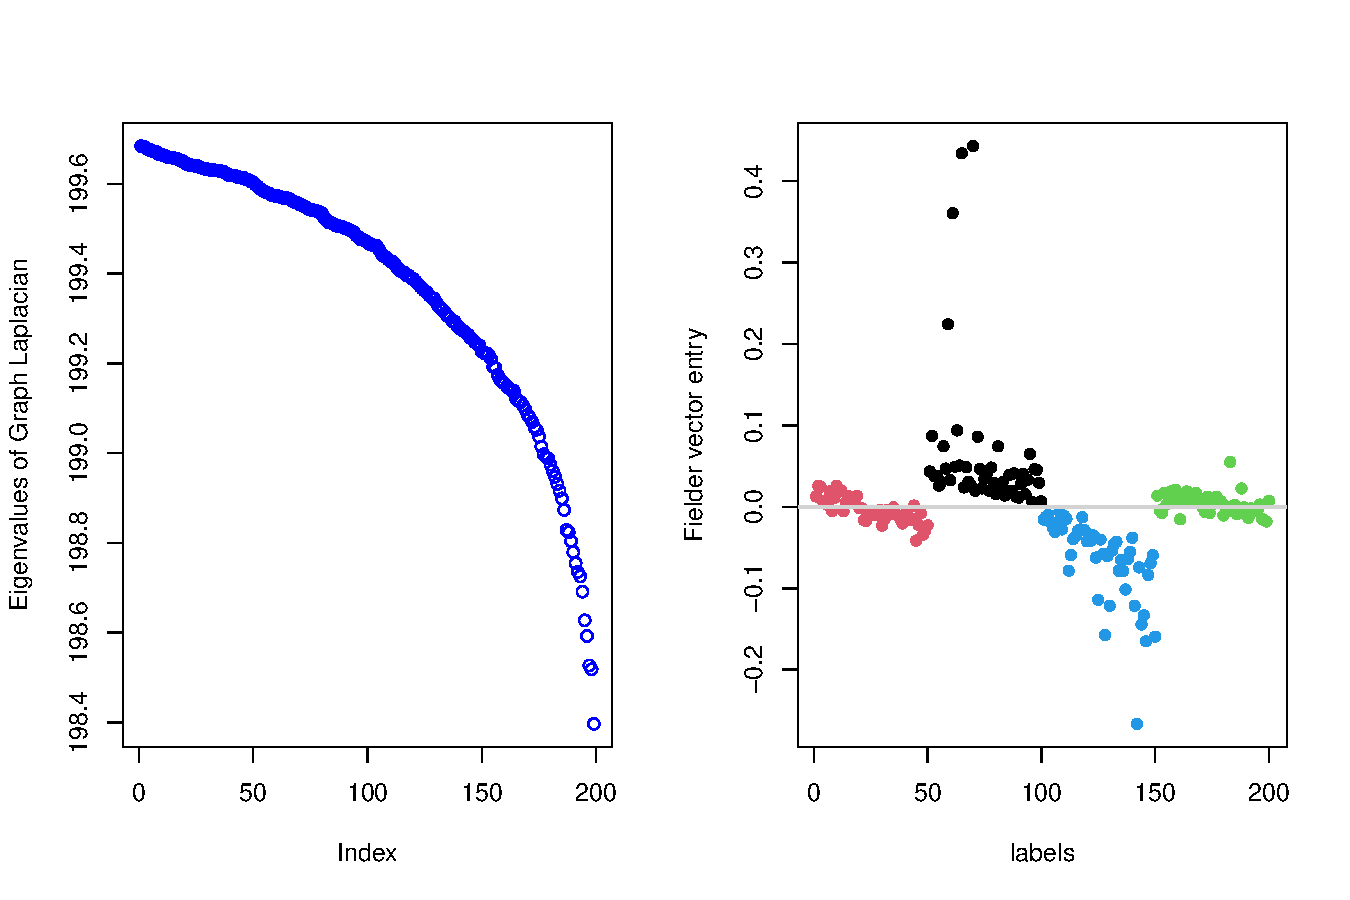
\includegraphics[width=.8\textwidth]{figures/laplacian_example-1} 

\end{knitrout}

\end{frame}

% \begin{frame}[fragile,allowframebreaks]
% 
% <<spectral clustering Gaussian kernel>>=
% sc_res <- crabs_corrected %>% select(-species, -sex) %>%  as.matrix() %>% 
%   specc(centers = 4, "rbfdot", sigma = 0.05)
% sc_clusters <- as.factor(sc_res)
% sc_centers  <- as.tibble(centers(sc_res))
% colnames(sc_centers)  <- colnames( crabs_corrected %>% select(-species, -sex))
% classes <- paste(crabs$species, crabs$sex, sep = "-")
% 
% crabs_corrected %>% 
%   ggplot(aes(x = carapace_length, y = carapace_width, color = sc_clusters)) +
%   geom_point(aes(shape = classes)) +
%   geom_point(data = sc_centers, color = 'coral', size = 4 , pch = 21) +
%   geom_point(data = sc_centers, color = 'coral', size = 50, alpha = 0.2)
% @
% 
% \end{frame}
% 
% \begin{frame}[fragile]
%   \frametitle{Clustering comparison}
% 
% <<sc validation>>=
% aricode::ARI(sc_clusters, classes)
% @
% 
% <<contingency_table_sc>>=
% knitr::kable(table(sc_clusters, classes),
% caption = "Estimating structure with spectral clustering, Gaussian kernel")
% @
% 
% \end{frame}
% 

\begin{frame}
  \frametitle{Some variants}

  \begin{definition}[(Normalized) Laplacian]
    The normalized Laplacian matrix $\bL$ is defined by 
    \[
      \bL_N = \bD^{-1/2}\bL\bD^{-1/2} = \bI - \bD^{-1/2} \bA \bD^{-1/2}.
    \]
  \end{definition}
  
  \vfill

  \begin{definition}[(Absolute) Graph Laplacian]
    The absolute Laplacian matrix $\bL_{abs}$ is defined by 
    \[
      \bL_{abs} = \bD^{-1/2}\bA\bD^{-1/2} = \bI - \bL_N,
    \]
    with eigenvalues $1-\lambda_n \leq \dots \leq 1-\lambda_2 \leq 1-\lambda_1 = 1$, where $0=\lambda_1\leq \dots \leq \lambda_n$ are the eigenvalues of $\bL_N$.
  \end{definition}

\end{frame}

\begin{frame}
  \frametitle{Normalized Spectral Clustering}
  \framesubtitle{by Ng, Jordan and Weiss (2002)}

\begin{algorithm}[H]
  \KwIn{Adjacency matrix and number of classes $Q$}
  \BlankLine\BlankLine
  \DontPrintSemicolon

  Compute the normalized graph Laplacian $\mathbf{L}$\;
  Compute the eigen vectors of $\mathbf{L}$ associated with the $Q$ \alert{smallest eigenvalues}\;
  Define $\mathbf{U}$,  the $n\times Q$ matrix  that encompasses these $Q$ vectors \;
  Define $\tilde{\mathbf{U}}$, the row-wise normalized version of $\mathbf{U}$: $ \tilde{u}_{ij} = \frac{u_{ij}}{\| \mathbf{U}_i\|_2}$\;
  Apply k-means to $(\tilde{\mathbf{U}}_i)_{i=1,\dots,n}$

  \BlankLine\BlankLine
  \KwOut{vector of classes $\mathbf{C}\in \mathcal{Q}^n$, such as  $C_i = q$ if $i\in q$}

\end{algorithm}

\end{frame}


\begin{frame}
  \frametitle{Absolute Spectral Clustering}
  \framesubtitle{by Rohe et al. (2011)}

\begin{algorithm}[H]
  \KwIn{Adjacency matrix and number of classes $Q$}
  \BlankLine\BlankLine
  \DontPrintSemicolon

  Compute the graph Laplacian $\mathbf{L}_{abs}$\;
  Compute the eigen vectors of $\mathbf{L}_{abs}$ associated with the $Q$ \alert{largest} absolute eigenvalues\;
  Define $\mathbf{U}$,  the $p\times Q$ matrix  that encompasses these $Q$ vectors \;
  Apply k-means to $(\mathbf{U}_i)_{i=1,\dots,p}$

  \BlankLine\BlankLine
  \KwOut{vector of classes $\mathbf{C}\in \mathcal{Q}^p$, such as  $C_i = q$ if $i\in q$}

\end{algorithm}

\end{frame}


\end{document}
